\documentclass[english,11pt,3p,number,sort&compress]{elsarticle}
\usepackage[T1]{fontenc}
\usepackage[latin9]{inputenc}
\usepackage{geometry}
\geometry{verbose,tmargin=2cm,bmargin=2cm,lmargin=2cm,rmargin=2cm,headheight=2cm,headsep=2cm,footskip=1cm}

\usepackage{color}
\usepackage{array}
\usepackage{float}
\usepackage{algorithm2e}
\usepackage{amsmath}
\usepackage{amssymb}
\usepackage{stmaryrd}
\usepackage{bm}
\usepackage{graphicx}
\usepackage{lipsum} 

%%%%%%%%%%%%%%%%%%%%%%%%%%%%%% LyX specific LaTeX commands.
%% Because html converters don't know tabularnewline
\providecommand{\tabularnewline}{\\}

%%%%%%%%%%%%%%%%%%%%%%%%%%%%%% User specified LaTeX commands.
%\usepackage[latin1]{inputenc}

\usepackage{natbib}
\usepackage{dsfont}
\usepackage{comment}
\usepackage{ifthen}    
\usepackage{lscape}
\usepackage{graphicx}
\usepackage{hyperref}

\usepackage[subpreambles=true]{standalone}
\usepackage{xspace}
\usepackage[percent]{overpic}

%tikz stuff
\usepackage[customcolors]{hf-tikz}
\usepackage{tikz}
\usepackage{pgfplots}
\usetikzlibrary{calc,shadings,patterns,tikzmark, plotmarks, spy, 
pgfplots.polar, external, matrix, shapes.symbols,shadings,shapes, 
decorations.shapes,decorations.pathmorphing,fit,backgrounds}
\pgfplotsset{compat=1.10}   %% <-- this added

\usepgfplotslibrary{groupplots}
\usetikzlibrary{calc}
\usepackage{pgfplotstable}

\usepackage{xcolor}

% WARNING: This folder must exist
\tikzexternalize[prefix=./figs_pgfplots/tikz/]

\newcommand{\includetikz}[1]{%
	\tikzsetnextfilename{#1}%
	\input{#1}%
}

% Commands for equations
\newcommand{\m}{\,\text{m}}

% compatibility for pgf figure
\pgfplotsset{compat=newest}

\hypersetup{urlcolor=blue, colorlinks=true}

% Useful when sending to journals.
% Do not provide path to figures in includegraphics comand. Set them
% here instead.
\graphicspath{ {./figs/} }

% path to tikz files. Do not use path in \includetikz command
\makeatletter
\def\input@path{{./figs_pgfplots/}{./figs/}}
\makeatother

\makeatletter
\@ifundefined{showcaptionsetup}{}{%
 \PassOptionsToPackage{caption=false}{subfig}}
\usepackage{subfig}
\makeatother

\usepackage{babel}

\newcommand{\giovane}{\color{red}{\bf\Large GA} \color{cyan} }
\newcommand{\nathan}{\color{red}{\bf\Large NS} \color{cyan} }
\newcommand{\phil}{\color{yellow}{\bf\Large PD} \color{cyan} }

\newcommand{\jump}[1]
{
	\llbracket #1 \rrbracket
}

\journal{Computer Methods in Applied Mechanics and Engineering}

\begin{document}

\begin{frontmatter}{}

%Um primeiro título
\title{A primal double-hybrid finite element method to solve tridimensional compressible, quasi-incompressible and incompressible elasticity using de Rham compatible H(div)-L2 spaces}

\author[uni]{Giovane Avancini}

\ead{giovanea@unicamp.br}

\author[uni]{Nathan Shauer}

\ead{shauer@unicamp.br}

\author[uni]{Hugo Luiz Oliveira}

\ead{hluiz@unicamp.br}

\author[uni]{Philippe R. B. Devloo}

\ead{phil@unicamp.br}

\address[uni]{Universidade Estadual de Campinas, R. Josiah Willard Gibbs 85 - Cidade Universitaria, Campinas SP, Brazil, CEP 13083-839}

%Definir se vamosar usar double-hybrid ou hybrid-hybrid. Adotei a segunda opção por enquanto
\begin{abstract}
	This work presents a novel primal double-hybrid finite element formulation for solving three-dimensional compressible, quasi-incompressible, and incompressible elasticity problems. Hybrid-mixed methods are typically derived from an extended variational principle, where interelement continuity requirements are relaxed and weakly enforced via Lagrange multipliers at element interfaces. In this context, we propose using a De Rham-compatible H(div)-L2 pair for displacements and pressure, respectively. The H(div) space naturally ensures normal displacement continuity across elements, while tangential continuity is recovered by introducing a shear stress approximation on element edges or faces, depending on the problem's dimension. This results in a semi-hybrid approach with two Lagrange multipliers, requiring the solution of a saddle-point problem even in the compressible regime. To overcome this drawback, hybridization is applied a second time to the shear stress which is statically condensed to recover a positive-definite block matrix that depends on the primal variable components. Although solving a saddle-point system remains necessary in the incompressible limit, numerical results demonstrate that this approach significantly enhances stability compared to the semi-hybrid formulation. Properties such as stability, consistency and local conservation are discussed in details. The formulation is tested and verified using 3D benchmarks for which analytical and/or numerical solutions are available, exhibiting optimal convergence rate, independent of the Poisson ratio. The proposed methodology is also applied to a real-world problem, where the robustness of the method is assessed.
\end{abstract}
\begin{keyword}
\textit{Mixed finite elements; Incompressible elasticity; H(div) approximation space; Hybridization}
\end{keyword}

\end{frontmatter}{}

\section{Introduction}

{\giovane A first shot, please give your contributions}
In the context of linear elasticity, several numerical methods have been developed in the past years. The most used one is the Finite Element Method (FEM). Using a continuous Galerkin approach to approximate the displacements may lead to shear-locking phenomenon due to spurious energy modes under bending \cite{bletzinger2000unified,belytschko1985stress} or volume-locking under quasi or full incompressibility, as the stresses go to infinity \cite{neto2005f,cervera2003mixed}.

There are different ways in the literature to overcome these drawbacks. One possible choice is to employ a mixed formulation \cite{brezzi2012mixed,arnold1988new} where the displacements and the stresses (or pressure) are approximated independently - i.e. the Taylor Hood elements \cite{taylor1973numerical} fulfill the \textit{inf-sup} condition yielding stable results for incompressible regime. This kind of approximation, on the other hand, is not locally conservative as it does not satisfy the divergence constraint in a strong manner. Another possibility is to use hybrid methods where the interelement continuity of a given field is broken and weakly imposed by means of a Lagrange multiplier (see for instance \cite{raviart1977primal,harder2016hybrid,farhloul1997dual}).

{\giovane escrevi esse texto na secao 5.1, mas ele fica melhor aqui.}In the context of Stokes-Brinkman flows, the authors in \cite{carvalho2024semi} developed a variant of the hybrid-mixed formulation that uses $H(\text{div},\Omega)$ velocity functions. In fact, the mixed problem of Eq. \eqref{eq:weak-mixed} and the hybrid version \eqref{eq:hybrid-weak} are stable, but none of them are locally conservative. This implies that, for Stokes flows, mass conservation does not hold strongly. Making a parallel to the incompressible elasticity, neither the incompressibility constraint is satisfied nor an equilibrated stress state is obtained element-wise.

In this work we extend the semi-hybrid approach proposed in \cite{carvalho2024semi} for Stokes flows to elasticity problems, developing a new formulation by performing a second hybridization on the tangential stresses. This formulation is based on a de Rham compatible pair $H(\text{div})-L^2$ for displacements and pressure. The $H(\text{div})$ functions are constructed using a systematic methodology described in \cite{devloo2022efficient,de2013new}.

\section{Preliminaries and notation}

Firstly, we shall introduce basic notation, functional spaces and definitions that will be used throughout this work. Elasticity problems involves scalar, vector and tensor valued variables. Hereinafter, vector fields are denoted by bold Latin letters, tensors are written using bold symbols or bold Greek letters, whislt plain Latin or Greek letters are chosen for scalars.

Let $\Omega \subset \mathbb{R}^d$, $d \in \{2, 3\}$, be a closed domain with Lipschitz boundary $\partial \Omega \subset \mathbb{R}^{d-1}$ whose  associated unit outward normal vector is denoted by $\bm{n}$. The scalar Hilbert spaces $L^2(\Omega)$ and $H^1(\Omega)$ have their usual meanings:
\begin{equation*}
    L^2(\Omega) = \left\{f: \int_{\Omega} f^2  ~d \Omega < \infty \right\},
\end{equation*}
\begin{equation*}
    H^1(\Omega) = \left\{v \in L^2(\Omega) : \partial_i v \in L^2 
    (\Omega) : i \in\{2,3\} \right\},
\end{equation*}

\noindent associated with their respective norms $\| \cdot \|_{L^2}$ and $\| \cdot \|_{H^1}$.

The space $H(\text{div},\Omega,\mathbb{R}^d)$ comprises square-integrable vector fields whose divergence is also square-integrable:
\begin{equation*}
	H(\text{div},\Omega,\mathbb{R}^d) = \left\{\bm{v} \in L^2(\Omega,\mathbb{R}^d) : \nabla \cdot \bm{v} \in L^2(\Omega) \right\},
\end{equation*}
\noindent equipped with the norm $\lVert \cdot \rVert_{H(\text{div})}$ and \(L^2(\Omega,\mathbb{R}^d)=\{\bm{v} : v_i \in L^2(\Omega) : i \in\{2,3\} \}\). 

The notation used for the $L^2$ inner product is $(\cdot,\cdot)_{\Omega}$, whilst $\langle \cdot,\cdot\rangle_{\partial\Omega}$ stands for the duality pairing between the trace spaces
\begin{equation*}
	H^{1/2}(\partial\Omega,\mathbb{R}^d) = \left\{\bm{v} \lvert_{\partial\Omega}, \bm{u} \in H^1(\Omega,\mathbb{R}^d)\right\},
\end{equation*}
\begin{equation*}
	H^{-1/2}(\partial\Omega,\mathbb{R}^d) = \left\{\bm{t}=\bm{\sigma} \,\bm{n} \lvert_{\partial\Omega}, \bm{\sigma} \in H(\text{div},\Omega,\mathbb{R}^d \times \mathbb{R}^d) \right\},
\end{equation*}

\noindent with $H(\text{div},\Omega,\mathbb{R}^d \times \mathbb{R}^d) = \left\{\bm{\sigma} \in L^2(\Omega,\mathbb{R}^{d \times d}) : \nabla \cdot \bm{\sigma} \in L^2(\Omega,\mathbb{R}^d) \right\}$ representing the space of tensor fields whose divergence is a vector field.

Let $\mathcal{T}_h=\left\{K_i \right\}, i\in \{1,...,N\}$ be a partition of $\Omega$ into non-overlapping elements $K$ with usual shape such that $\Omega = \cup_{i=1}^{N} K_i$. The boundary of each element is denoted by $\partial K$ with outward unit normal vector to the boundary $\bm{n}^K$. The set $\Gamma_h=\cup_{K \in \mathcal{T}_h} \partial K$ is named the mesh skeleton, and comprises the union of all element boundary segments (lines for 2D and facets for 3D). It can be decomposed into a boundary subset $\Gamma_{\partial\Omega}=\{E \in \Gamma_h : E \subset \partial\Omega\}$ and an interior subset $\mathring{\Gamma}_h =\{E \in \Gamma_h \setminus \Gamma_{\partial\Omega}\}$. Analogously, $\partial\mathcal{T}_h=\bigcup_{K \in \mathcal{T}_h} \partial K$ denotes the disjoint union of all element boundaries. Note that $\Gamma_h$ differs from $\partial\mathcal{T}_h$ since for every $E \in \mathring{\Gamma}$, the latter includes the boundaries from both adjacent elements.

Over an element interface $E \in \mathring{\Gamma}_h$ between two elements $K_i$ and $K_j$, the jump operator of a function $v$ is defined as
\begin{equation*}
	\jump{v}_E = v_i \lvert_{E} - v_j \lvert_{E} \text{.}
\end{equation*}

Moreover, a broken Sobolev space of the square-integrable functions on the discretized domain can be defined as
\begin{equation*}
	X(\mathcal{T}_h) = \left\{v \in L^2(\Omega) : v \lvert_{K} \in H^1(K), \,\forall \, K\in\mathcal{T}_h \right\} ,
\end{equation*}

\noindent and the space of functions whose trace normal component is continuous across elements is denoted by
\begin{equation*}
	\mathcal{V}(\mathcal{T}_h,\mathbb{R}^d) = X(\mathcal{T}_h,\mathbb{R}^d) \cap H(\text{div},\Omega) .
\end{equation*} 

{\giovane Acho que, ao contrario do artigo do Stokes, vou colocar os espacos discretos conforme eles forem aparecendo nas secoes.}

\section{Elasticity problem \label{sec:Governing-equations}}

In this section, the governing equations for the linear elasticity problem shall be defined. Firstly, the primal displacement based formulation is presented, followed by the mixed version introducing the pressure as an indepent variable.

\subsection{Problem definition}

The conservation of linear momentum for a generic continuum body is given by:
\begin{equation} \label{eq:momentum}
		-\nabla \cdot \bm{\sigma} - \bm{b} = \bm{0} \hspace{0.2cm} \text{in } \Omega ,
\end{equation}
\noindent where $\bm{b}$ is the body forces vector and $\bm{\sigma}$ denotes the Cauchy stress tensor. The Generalized Hook law relates the stresses and strains in a isotropic body as:
\begin{equation} \label{eq:hook}
    \bm{\sigma} = 2\mu \bm{\varepsilon}(\bm{u}) + \lambda \text{tr}(\bm{\varepsilon}(\bm{u})) \bm{I}^d ,
\end{equation}

\noindent where $\mathbf{I}^d$ is the identity tensor of dimension $d$, $\mu$ and $\lambda$ are scalars known as Lam\'{e} constants, given respectively by
\begin{equation}
	\lambda = \frac{E\nu}{(1+\nu)(1-2\nu)} \text{,} \quad \mu = \frac{E}{2(1+\nu)} \text{,}
\end{equation}

\noindent with $E$ and $\nu$ standing for the Young modulus and Poisson coefficient. The infinitesimal strain tensor $\bm{\varepsilon}(\bm{u})$ is the symmetric countepart of the displacement gradient:
\begin{equation} \label{eq:strain}
    \bm{\varepsilon}(\bm{u})=\frac{1}{2}(\nabla\bm{u}^T+\nabla\bm{u}) \text{.}
\end{equation}

By substituting Eqs. \eqref{eq:hook} and \eqref{eq:strain} into Eq. \eqref{eq:momentum}, the pure displacement boundary value problem, also known as the Navier-Cauchy problem, reads: find displacement $\bm{u}$ such that
\begin{subequations} \label{eq:navier-cauchy}
	\begin{align}
		-\mu\nabla^2\bm{u} -\left(\mu+\lambda \right)\nabla\left(\nabla \cdot \bm{u} \right) - \bm{b} = \bm{0} \hspace{0.2cm} \text{in } \Omega ,&\\
		\bm{u} = \bm{u}_D \hspace{0.2cm} \text{on } \partial\Omega_D ,&\\
		\bm{\sigma} \mathbf{n} = \bm{t}_N \hspace{0.2cm} \text{on } \partial\Omega_N ,&
	\end{align}
\end{subequations}

\noindent where $\bm{u}_D$ and $\bm{t}$ are the prescribed displacements and tractions on the Dirichlet $\partial\Omega_D$ and Neumann $\partial\Omega_N$ boundaries, respectively.

The elasticity problem can also be formulated using two state variables by applying the additive decomposition on the Cauchy stress tensor in its deviatoric and hydrostatic counterparts, resulting in:
\begin{equation} \label{eq:stress-decomposition}
	\bm{\sigma} = \bm{\sigma}' - p\bm{I}^d ,
\end{equation}

\noindent where the scalar p is the hydrostatic pressure, computed as
\begin{equation} \label{eq:pressure}
	p = -\kappa \text{tr}(\bm{\varepsilon}(\bm{u})) ,
\end{equation}

\noindent with $\kappa$ standing for the bulk modulus, which for the generalized tridimensional case, is computed as $\kappa=\frac{2\mu+3\lambda}{3}$. Its value for the plane stress and plane strain hypothesis can also be derived by imposing the constraints on each case {\giovane should we put the derivation of the bulk modulus for the plane analyses in an appendix?}. Plugging Eqs. \eqref{eq:pressure} and \eqref{eq:hook} into Eq. \eqref{eq:stress-decomposition}, the deviatoric stress tensor $\boldsymbol{\sigma}'$ is computed as:
\begin{equation} \label{eq:deviatoric-stress}
	\boldsymbol{\sigma}' = 2\mu \left(\boldsymbol{\varepsilon}(\bm{u}) - \frac{1}{3}\text{tr}(\boldsymbol{\varepsilon}(\bm{u}))\mathbf{I}\right) \text{.}
\end{equation}

Substituting Eqs. \eqref{eq:stress-decomposition}, \eqref{eq:pressure}, \eqref{eq:deviatoric-stress} in Eq. \eqref{eq:momentum}, the mixed elasticity problem yields: find $\mathbf{u}$ and $p$ such that
\begin{subequations} \label{eq:mixed-elasticity}
	\begin{align}
		-\mu\nabla^2\bm{u} -\frac{2}{3}\mu\nabla\left(\nabla \cdot \bm{u} \right) + \nabla p -\bm{b}= \bm{0} \hspace{0.2cm} \text{in } \Omega ,& \label{eq:mixed-elasticity-a}\\ 
		-\nabla \cdot \bm{u} -\frac{1}{\kappa}p= 0 \hspace{0.2cm} \text{in } \Omega ,& \label{eq:mixed-elasticity-b}\\ 
		\bm{u} = \bm{u}_D \hspace{0.2cm} \text{on } \partial\Omega_D ,&\\
		\bm{\sigma} \bm{n} = \bm{t}_N \hspace{0.2cm} \text{on } \partial\Omega_N .&
	\end{align}
\end{subequations}

\subsection{Weak form}

The weak form of the problems described by Eqs. \eqref{eq:navier-cauchy} and \eqref{eq:mixed-elasticity} can be obtained by means of the weighted residual method. Depending on the choice of test functions and approximation spaces, different formulations can be derived.

The simplest one is obtained by multiplying Eq. \eqref{eq:navier-cauchy} by test functions $\bm{v} \in H^1_0(\Omega,\mathbb{R}^d)$, where $H^1_0(\Omega,\mathbb{R}^d)=\{\bm{v} \in H^1(\Omega,\mathbb{R}^d) : \bm{v} \lvert_{\partial\Omega_D}=0 \}$ and integrating over the domain $\Omega$ \cite{becker1981finite}. The weak statement then reads: find $\mathbf{u} \in H^1_D(\Omega,\mathbb{R}^d)$ such that for all $\mathbf{v} \in H^1_0(\Omega,\mathbb{R}^d)$:
\begin{equation} \label{eq:weak-primal-displacement}
    a\left(\bm{u},\bm{v}\right)_\Omega = \left(\bm{b},\bm{v}\right)_\Omega + \langle\bm{t}_N,\bm{v}\rangle_{\partial\Omega_N},
\end{equation}
% \begin{equation} \label{eq:weak-primal-displacement}
%     \int_{\Omega} \boldsymbol{\varepsilon}(\mathbf{v}) : \mathcal{D} : \boldsymbol{\varepsilon}(\mathbf{u}) d\Omega = \int_{\Omega} \mathbf{v} \cdot \mathbf{b} d\Omega + \int_{\partial\Omega_N} \mathbf{v} \cdot \mathbf{t} \;d\partial\Omega \text{.}
% \end{equation}

\noindent where $H^1_D(\Omega,\mathbb{R}^d)=\{\bm{u} \in H^1(\Omega,\mathbb{R}^d) : \bm{u} \lvert_{\partial\Omega_D}=\bm{u}_D\}$, $a\left(\bm{u},\bm{v}\right)_\Omega$ is a bilinear operator computed as
\begin{equation*}
	a\left(\bm{u},\bm{v}\right)_\Omega = \int_{\Omega} \bm{\varepsilon}(\bm{v}) : \mathcal{D} : \bm{\varepsilon}(\bm{u}) d\Omega
\end{equation*}

In the above equations, $\mathcal{D}$ refers to the elasticity constitutive tensor, defined for an isotropic solid as $\mathcal{D}_{ijkl} = \mu(\delta_{ik}\delta_{jl}+\delta_{il}\delta_{jk})+\lambda\delta_{ij}\delta_{kl}$, where $\delta_{ij}$ is the Kronecker delta, and $:$ is a double contraction operator i.e. $\bm{\sigma}:\bm{\varepsilon} = \sigma_{ij}\varepsilon_{ji}$. Equation \eqref{eq:weak-primal-displacement} is the starting point for the $H^1$ primal displacement based finite element formulations.

In order to derive the weak form of the mixed problem from Eq. \eqref{eq:mixed-elasticity}, we multiply Eq. \eqref{eq:mixed-elasticity-a} by displacement test functions $\bm{v} \in H^1_0(\Omega,\mathbb{R}^d)$ and the Eq. \eqref{eq:mixed-elasticity-b} by pressure test functions $q \in L^2(\Omega)$. Integrating over the domain $\Omega$ and applying the divergence theorem, the weak form consists in finding $\bm{u} \in H^1_D(\Omega,\mathbb{R}^d)$ and $p \in L^2(\Omega)$ such that for all $\bm{v} \in H^1_0(\Omega)$ and $q \in L^2(\Omega)$:
\begin{subequations} \label{eq:weak-mixed}
	\begin{align}
		a\left(\bm{u},\bm{v}\right)_\Omega - b\left( p, \bm{v}\right)_\Omega &= \left(\bm{b},\bm{v}\right)_\Omega + \langle\bm{t}_N,\bm{v}\rangle_{\partial\Omega_N} ,\label{eq:weak-mixed-a}\\ 
		-b\left(\bm{u}, q\right)_\Omega - c\left(p,q \right)_\Omega &= 0 . \label{eq:weak-mixed-b}
	\end{align}
\end{subequations}

% \begin{equation} \label{eq:weak-mixed1}
% 	\int_{\Omega} \boldsymbol{\varepsilon}(\mathbf{v}) : \mathcal{D}^{'} : \boldsymbol{\varepsilon}(\mathbf{u}) d\Omega - \int_{\Omega_e} p \;(\nabla \cdot \mathbf{v}) d\Omega =  \int_{\Omega} \mathbf{v} \cdot \mathbf{b} d\Omega + \int_{\partial\Omega_N} \mathbf{v} \cdot \mathbf{t} \;d\partial\Omega \text{,}
% \end{equation}
% \begin{equation} \label{eq:weak-mixed2}
% -\int_{\Omega} (\nabla \cdot \mathbf{u}) \;q\; d\Omega -\int_{\Omega} \frac{1}{\kappa}\;p \;q\; d\Omega = \mathbf{0} \text{,}
% \end{equation}
\noindent Here, the bilinear forms are computed as
\begin{equation*}
	a\left(\bm{u},\bm{v}\right)_\Omega = \int_{\Omega} \bm{\varepsilon}(\bm{v}) : \mathcal{D}^{'} : \bm{\varepsilon}(\bm{u}) d\Omega ,
\end{equation*}
\begin{equation*}
	b\left(p, \bm{v}\right)_\Omega = \int_{\Omega} p \,\nabla \cdot \bm{v} \, d\Omega ,
\end{equation*}
\begin{equation*}
	c\left(p,q \right)_\Omega = \int_{\Omega} \frac{1}{\kappa} \,p \,q \, d\Omega ,
\end{equation*}

\noindent where $\mathcal{D}^{'}$ stands for the deviatoric part of the elasticity constitutive tensor, computed as $\mathcal{D}^{'}_{ijkl} = \mu(\delta_{ik}\delta_{jl}+\delta_{il}\delta_{jk})-\frac{2}{3}\mu\delta_{ij}\delta_{kl}$. Eqs. \eqref{eq:weak-mixed-a}-\eqref{eq:weak-mixed-b} give rise to a saddle point problem with pressure playing the role as a Lagrange multiplier. When the material approaches the incompressible regime, i.e. $\nu \rightarrow 0.5$, the system becomes ill conditioned and the choice for the approximation spaces used for displacement and pressure must follow a specific criteria to ensure stability. A stable solution can be obtained if the Ladyzhenskaya-Babuska-Brezzi (LBB) condition is satisfied \cite{brezzi2012mixed}, that is, there exist a constant $\beta>0$ such that
\begin{equation*}
	\inf_{q \in L^2,q\neq0} \sup_{\bm{v} \in H^1_0,\bm{v}\neq\bm{0}} \frac{b\left(\bm{v},q\right)}{\|\bm{v}\|_{H^1} \|q\|_{L^2}} \geq \beta .
\end{equation*}

\noindent A convenient choice that fulfills this requirement is the Taylor-Hood elements \cite{taylor1973numerical} described in Section \ref{sec:taylor-hood}.

\section{Mixed displacement-pressure Taylor Hood elements \label{sec:taylor-hood}}

Let $\mathbb{Q}_k(K)$ represent the space of scalar polynomial functions of order $k$ over an element $K\in\mathcal{T}_h$. For vector functions, the notation $\mathbb{Q}_k(K,\mathbb{R}^d)$ is used. For the Taylor-Hood element, the discrete FE spaces used for displacement and pressure are defined, respectively, by:
\begin{equation}
    \label{eq:uTH}
    \mathcal{U}_k(\mathcal{T}_h,\mathbb{R}^d) = \left\{\bm{v} \in H^1(\Omega,\mathbb{R}^d) : \bm{v}\lvert_{K} \in \mathbb{Q}_k(K,\mathbb{R}^d), \,\forall \,K \in \mathcal{T}_h, \, k\geq 2 \right\}.
\end{equation}
\begin{equation}
    \label{eq:qTH}
    \mathcal{Q}_k(\mathcal{T}_h) = \left\{q \in H^1(\Omega) \,:\, q\lvert_{K} \, \in \mathbb{Q}_{k-1}(K), \,\forall \, K \in \mathcal{T}_h, \, k\geq 2\right\},
\end{equation}

For the forthcoming FE spaces whose boundary conditions need to be enforced directly in the space, it is convenient to perform a decomposition into homogeneous and non-homogeneous counterparts as follows:
\begin{equation}
    \label{eq:uTH0}
    \mathcal{U}^0_k(\mathcal{T}_h,\mathbb{R}^d)=\left\{ \bm{v} \in \mathcal{U}_k(\mathcal{T}_h,\mathbb{R}^d) : \bm{v} \lvert_{\partial\Omega_D}=\bm{0}\right\},
\end{equation}
\begin{equation}
    \label{eq:uTHD}
    \mathcal{U}^D_k(\mathcal{T}_h,\mathbb{R}^d)=\left\{ \bm{v} \in \mathcal{U}_k(\mathcal{T}_h,\mathbb{R}^d) : \bm{v} \lvert_{\partial\Omega_D}=\bm{u}_D\right\}.
\end{equation}

\noindent Hereinafter, the superscripts $(\cdot)^0$ and $(\cdot)^D$ refer to this type of decomposition. Throughout this paper, the notation $P_k P_{k-1}$ is used to denote the pair $\mathcal{U}_k \times \mathcal{Q}_k$ when referring to a specific Taylor-Hood element.

Then, the discretized mixed elasticity problem of Eq. \eqref{eq:mixed-elasticity} using Taylor-Hood elements is formulated is follows: find $\{\bm{u},p\}$ $\in \mathcal{U}^D_k \times \mathcal{Q}_k$ such that
\begin{subequations} \label{eq:TH-weak}
	\begin{align}
		a\left(\bm{u},\bm{v}\right)_{\mathcal{T}_h} - b\left( p, \bm{v}\right)_{\mathcal{T}_h} &= \left(\bm{b},\bm{v}\right)_{\mathcal{T}_h} + \langle\bm{t}_N,\bm{v}\rangle_{\partial\Omega_N} ~~\forall\, \bm{v} \in \mathcal{U}^0_k,\label{eq:TH-weak-a}\\ 
		-b\left(\bm{u}, q\right)_{\mathcal{T}_h} - c\left(p,q \right)_{\mathcal{T}_h} &= 0 ~~\forall\, q \in \mathcal{Q}_k, \label{eq:TH-weak-b}
	\end{align}
\end{subequations}

\noindent where the discretized operators are:
\begin{equation*}
	a\left(\bm{u},\bm{v}\right)_{\mathcal{T}_h} = \sum_{K \in \mathcal{T}_h} \int_{K} \bm{\varepsilon}(\bm{v}) : \mathcal{D}^{'} : \bm{\varepsilon}(\bm{u}) dK ,
\end{equation*}
\begin{equation*}
	b\left(p, \bm{v}\right)_{\mathcal{T}_h} = \sum_{K \in \mathcal{T}_h} \int_{K} p \,\nabla \cdot \bm{v} \, dK ,
\end{equation*}
\begin{equation*}
	c\left(p,q \right)_{\mathcal{T}_h} = \sum_{K \in \mathcal{T}_h} \int_{K} \frac{1}{\kappa} \,p \,q \, dK ,
\end{equation*}
\begin{equation*}
	\left(\bm{b},\bm{v}\right)_{\mathcal{T}_h} = \sum_{K \in \mathcal{T}_h} \int_{K} \bm{v} \cdot \bm{b} \, dK ,
\end{equation*}
\begin{equation*}
	\langle\bm{t}_N,\bm{v}\rangle_{\partial\Omega_N} = \sum_{E \in \partial\Omega_N} \int_{E} \bm{t}_N \cdot \bm{v} \, d\partial K .
\end{equation*}

In this approach, displacements are strongly imposed on the Dirichlet boundary $\partial \Omega_D$ through the restricted space $\mathcal{U}^D_k$ whilst surface tractions are weakly imposed on the boundary $\partial \Omega_N$ in the right-hand side of Eq. \eqref{eq:TH-weak-b}.

\section{Hybrid-mixed formulations}

The mixed problem of Eq. \eqref{eq:weak-mixed} can be presented in an alternative way by relaxing the continuity requirement of the displacement functions across elements. Let define the space of the stress traces over the mesh skeleton as
\begin{equation}
	\label{eq:space-traction}
	\mathcal{L}(\Gamma_h,\mathbb{R}^d) = \left\{\bm{t} \in H^{-1/2}(\Gamma_h,\mathbb{R}^d), \, \bm{t}=\bm{\sigma}\bm{n}\lvert_{\partial K}, \, \forall \, E \in \Gamma_h ~:~\bm{\sigma} \in H(\text{div},\Omega,\mathbb{R}^d \times \mathbb{R}^d) \right\}.
\end{equation}

Then, a hybrid-mixed problem is derived by finding $\{\bm{u},p,\bm{t}\} \in X^D \times L^2 \times \mathcal{L}^N$ such that:
\begin{subequations} \label{eq:hybrid-weak}
	\begin{align}
		a\left(\bm{u},\bm{v}\right)_{\mathcal{T}_h} - b\left( p, \bm{v}\right)_{\mathcal{T}_h} -\langle\bm{t},\jump{\bm{v}}\rangle_{\Gamma_h} &= \left(\bm{b},\bm{v}\right)_{\mathcal{T}_h} ~~\forall\, \bm{v} \in X^0,\label{eq:hybrid-weak-a}\\ 
		-b\left(\bm{u}, q\right)_{\mathcal{T}_h} - c\left(p,q \right)_{\mathcal{T}_h} &= 0 ~~\forall\, q \in L^2, \label{eq:hybrid-weak-b}\\
		-\langle\jump{\bm{u}},\bm{z}\rangle_{\Gamma_h} &= 0 ~~\forall\, \bm{z} \in \mathcal{L}^0, \label{eq:hybrid-weak-c}
	\end{align}
\end{subequations}

\noindent where the spaces $\mathcal{L}^0$ and $\mathcal{L}^N$ can be written using the same notation as in Eqs. \eqref{eq:uTH0} and \eqref{eq:uTHD} but restricted on $\partial\Omega_N$. The new traction variable $\bm{t}$ acts as a Lagrange multiplier weakly imposing the displacement continuity over the discretized domain.

The equivalence of problems described in Eq. \eqref{eq:hybrid-weak} and Eq. \eqref{eq:weak-mixed} was proven in \cite{raviart1977primal}. The hybridization technique is often used to improve the conditioning and spectral properties of the system matrix, and we will explore this feature in the following sections \cite{arnold1985mixed}.

\subsection{Semi-hybrid formulation using \(H(\text{div},\Omega)\) approximation space}

In \cite{carvalho2024semi}, the authors proposed a variant of the hybrid-mixed formulation for Stokes-Brinkman flows that uses \(H(\text{div})\) functions to approximate velocities. As a consequence, the normal component of its trace is continuous between adjacent elements, meaning that only the continuity requirement of the tangential component is weakened compared to $H^1(\Omega)$-conforming methods. We show next that its extension to elasticity is straightforward.

Firstly, the traction $\bm{t} \in \mathcal{L}$ can be decomposed into normal and tangential components $\bm{t} = \bm{t}^n + \bm{t}^t$, so we write the decomposed spaces as:

\begin{subequations}
	\begin{align}
		\mathcal{L}^n(\Gamma_h,\mathbb{R}^d) &= \left\{\bm{t}^n=((\bm{t}\cdot\bm{n})\bm{n})\lvert_{\partial K}, ~\bm{t} \in \mathcal{L}(\Gamma_h,\mathbb{R}^d) \right\}\label{eq:space-traction-normal}\\
		\mathcal{L}^t(\Gamma_h,\mathbb{R}^d) &= \left\{\bm{t}^t=\bm{t}-\bm{t}^n, ~\bm{t} \in \mathcal{L}(\Gamma_h,\mathbb{R}^d) \right\}\label{eq:space-traction-tangential}
	\end{align}
\end{subequations}




, the authors proposed a semi-hybrid formulation for Stokes-Brinkman flows that uses $H(\text{div})$ conforming velocity functions and discontinuos $L^2$ approximation for pressure. The same ideia can also be applied to elasticity. Let $\mathcal{V} = \mathbf{V}\cap H(\text{div},\Omega)$, $\Psi \subset L^2(\Omega)$ be spaces of vector functions and piece-wise scalars, respectively, for which the relation $\nabla \cdot \mathcal{V} \in \Psi$ holds. As $H(\text{div})$ approximation only guarantees the continuity of normal componentes of a vector across elements interface, a hybridization of the tangential velocity is performed. We introduce a third space defined as $\boldsymbol{\Lambda}^t \subset H^{-1/2}(\partial\Omega_e)$, for which the Lagrange multiplier $\boldsymbol{\lambda}^t \in \boldsymbol{\Lambda}^t$ has the meaning of a shear traction to weakly enforce the tangential displacement continuity. 

Moreover, we set a discontinuous pressure space
\begin{equation}
	\mathcal{P}(\mathcal{T}_h) = \{q \, \in L^2(\Omega) ~\lvert~ q\lvert_K \in \mathbb{Q}_k(K) ~:~ \forall K \in \mathcal{T}_h\}
\end{equation}
\noindent which admits the following decomposition $\mathcal{P}=\bar{\mathcal{P}} \oplus \mathcal{P}^\perp$, where $\mathcal{P}$ stands for piece-wise constant functions over $\mathcal{T}_h$ and $\mathcal{P}^\perp$ is the piece-wise zero-mean functions over $\mathcal{T}_h$.

The weak statement for the semi-hybrid formulation thus reads: find $\{\mathbf{u},p,\boldsymbol{\lambda}^t\} \in \mathcal{V} \times \Psi \times \boldsymbol{\Lambda}^t$ such that for all $\{\mathbf{v},q,\boldsymbol{\eta}^t\} \in \mathcal{V}\times \Psi \times \boldsymbol{\Lambda}^t$:

\begin{equation} \label{eq:semihybrid1}
    \begin{split}
        \sum_{\Omega_e \in \mathcal{T}} \left( \int_{\Omega_e} \boldsymbol{\varepsilon}(\mathbf{v}) : \mathcal{D}^{'} : \boldsymbol{\varepsilon}(\mathbf{u}) d\Omega_e - \int_{\Omega_e} p\; (\nabla \cdot \mathbf{v}) d\Omega_e \right) + \int_{\mathcal{E}^0} \boldsymbol{\lambda}^t \cdot \llbracket \mathbf{v} \rrbracket \;d\mathcal{E}^0 = \\ \sum_{\Omega_e \in \mathcal{T}} \left( \int_{\Omega_e} \mathbf{v} \cdot \mathbf{b} d\Omega_e + \int_{\Gamma} \mathbf{v} \cdot \boldsymbol{\sigma}_N \; d\partial\Omega_e \right)
    \end{split}
\end{equation}
\begin{equation} \label{eq:semihybrid2}
    \sum_{\Omega_e \in \mathcal{T}} \left(-\int_{\Omega_e} (\nabla \cdot \mathbf{u}) \;q\; d\Omega_e -\int_{\Omega_e} \frac{3}{2\mu+\lambda}\;p\; q\; d\Omega_e \right) = \mathbf{0}
\end{equation}
\begin{equation} \label{eq:semihybrid3}
    \int_{\mathcal{E}^0} \llbracket \mathbf{u} \rrbracket \cdot \mathbf{\eta}^t \;d\mathcal{E}^0 = \mathbf{0} \text{,}
\end{equation}

\noindent where $\mathbf{v}$, $q$ and $\boldsymbol{\eta}^t$ are test functions for velocity, pressure and tangential traction, respectively, $\llbracket \cdot \rrbracket$ stands for the jump operator on the interface $\mathcal{E}^0$ between two neighbour elements $\Omega_1$ and $\Omega_2$, defined as $\llbracket \mathbf{v} \rrbracket = \mathbf{v} \vert_{\Omega_1} - \mathbf{v} \vert_{\Omega_2}$. Equation \eqref{eq:semihybrid3} plays the role of weakly enforcing the tangential displacement continuity over the element interfaces.

Although mathematically consistent, the semi-hybrid formulation poses some challenges from a numerical perspective. It gives rise to a saddle-point problem with two different constraints: $p$ and $\boldsymbol{\lambda}^t$. This structure significantly increases the efforts required to consistently and stably solve the linear system.

We propose a second hybridization of the tangential stresses in order to recover its primal form. Introducing the space $\mathcal{L}^t \subset H^{1/2}(\partial\Omega_e)$ for the tangential velocity, the hybrid form thus reads: find $\{\mathbf{u},p,\boldsymbol{\lambda}^t_e,\mathbf{u}^t\} \in \mathcal{V} \times \Psi \times \boldsymbol{\Lambda}^t \times \mathcal{L}^t$ such that for all $\{\mathbf{v},q,\boldsymbol{\eta}^t_e,\mathbf{v}^t\} \in \mathcal{V} \times \Psi \times \boldsymbol{\Lambda}^t\times \mathcal{L}^t$, the following equations are satisfied:

\begin{equation} \label{eq:hybrid1}
    \begin{split}
        \sum_{\Omega_e \in \mathcal{T}} \left( \int_{\Omega_e} \boldsymbol{\varepsilon}(\mathbf{v}) : \mathcal{D}^{'} : \boldsymbol{\varepsilon}(\mathbf{u})\; d\Omega_e - \int_{\Omega_e} p \;(\nabla \cdot \mathbf{v}) d\Omega_e - \int_{\partial\Omega_e} \boldsymbol{\lambda}^t_e \cdot \mathbf{v}\; d\partial\Omega_e \right) = \\ \sum_{\Omega_e \in \mathcal{T}} \left( \int_{\Omega_e} \mathbf{v} \cdot \mathbf{b} \;d\Omega_e + \int_{\Gamma} \mathbf{v} \cdot \boldsymbol{\sigma}_N\; d\partial\Omega_e \right)
    \end{split}
\end{equation}
\begin{equation} \label{eq:hybrid2}
    \sum_{\Omega_e \in \mathcal{T}} \left(-\int_{\Omega_e} (\nabla \cdot \mathbf{u})\; q \;d\Omega_e -\int_{\Omega_e} \frac{3}{2\mu+\lambda}\;p \;q \;d\Omega_e \right) = \mathbf{0}
\end{equation}
\begin{equation} \label{eq:hybrid3}
    \sum_{\Omega_e \in \mathcal{T}} \left(\int_{\partial\Omega_e} (\mathbf{u}^t-\mathbf{u}) \cdot \boldsymbol{\eta}^t_e\; d\partial\Omega_e \right)  = \mathbf{0}
\end{equation}
\begin{equation} \label{eq:hybrid4}
    \sum_{\Omega_e \in \mathcal{T}} \int_{\partial\Omega_e} \boldsymbol{\lambda}^t_e \cdot \mathbf{v}^t\; d\partial\Omega_e = \mathbf{0} \text{,}
\end{equation}

\noindent where Eq. \eqref{eq:hybrid4} was introduced to impose the continuity of the tangential traction across $\mathcal{E}^0$. Even though an additional constraint is introduced, $\boldsymbol{\lambda}^t$ is now associated to a single element therefore it can be statically condensed and eliminated from the global system. For a compressible solid, a symmetric positive-definite matrix is obtained with two unknowns, namely $\mathbf{u} \in H(\text{div},\Omega)$ and $\mathbf{u}^t \in H^{1/2}(\partial\Omega_e)$. For the incompressible case where pressures cannot be computed explicitly from the displacements, one mean pressure per element acts as a Lagrange multiplier in the global system. This still gives rise to a saddle-point matrix, however, with much better spectral properties and easier to solve compared to Eqs. \eqref{eq:semihybrid1}-\eqref{eq:semihybrid3}.

\subsection{Comparison with H1-hybrid formulation}

{\giovane O Phil trabalhou nisso na China, talvez ele poderia escrever essa parte?}
\lipsum[1-1]

\subsection{Static condensation of the internal degrees of freedom}

{\giovane Separei o material para essa parte. Voltarei em 29/01}

\section{Examples \label{sec:Examples}}

In this section, the proposed methodology is tested and verified through three benchmarks for which analytical and/or numerical solutions are available and a real-world problem. In the first case, a non-homogeneous solid under pure stretch is analyzed to show the advantage of the hybrid formulation to represent stress discontinuities over element interfaces in comparison to the Taylor-Hood scheme. In the second example, a cantilever beam is investigated in different compressibility regime to show the independency of the convergence rate to the poisson coefficient. Next, the classical Cook's membrane problem is solved, followed by a real-world problem where the applicability of the method is demonstrated.

\subsection{Uniform stretch of a non-homogeneous solid \label{subsec:non-homogeneous}}

{\giovane to do next}

\subsection{Cantilever beam subjected to an end shear load \label{subsec:bishop}}

The case of a tridimensional cantilever beam under an end shear-load is considered. Its initial geometry is depicted in Figure \ref{fig:bishop-beam-geometry}, with $L=5$, $a=0.5$, $b=0.5$. The beam is assumed to be fixed at $z=0$ and subjected to a shear-force $F=1$ at $z=L$ pointing downwards in the $y$ direction, while the other faces are traction-free. The material is assumed to have a linear isotropic behaviour with a constant Young modulus $E=1$ whereas different values are used for the poisson coefficient in order to test the formulation for a wide range of compressibility.

\begin{figure}[H]
	\centering
	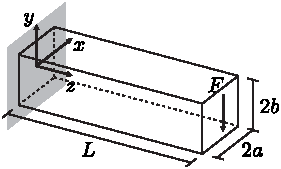
\includegraphics[scale=1.0]{bishop-beam-geometry}
	\caption{Cantilever beam subjected to an end shear load - geometry}
	\label{fig:bishop-beam-geometry}
\end{figure}

The analytical stress state for the problem is given in \cite{bishop2014displacement} and written below:

\begin{equation} \label{eq:bishop-stress}
	\begin{aligned}
		\sigma_{xx} &= \sigma_{xy} = \sigma_{yy} = 0 \text{,}\\
		\sigma_{zz} &= \frac{F}{I} yz \text{,}\\
		\sigma_{xz} &= \frac{F}{I} \frac{2a^2}{\pi^2}\frac{\nu}{1+\nu} \sum_{n=1}^{\infty} \frac{(-1)^n}{n^2} \text{sin}\left(n\pi x/a\right) \frac{\text{sinh}\left( n\pi y/a \right)}{\text{cosh}\left( n\pi b/a \right)} \text{,}\\
		\sigma_{yz} &= \frac{F}{I} \frac{b^2-y^2}{2} + \frac{F}{I}\frac{\nu}{1+\nu} \left[ \frac{3x^2-a^2}{6} - \frac{2a^2}{\pi^2} \sum_{n=1}^{\infty} \frac{(-1)^n}{n^2} \text{cos}\left(n\pi x/a\right) \frac{\text{cosh}\left( n\pi y/a \right)}{\text{cosh}\left( n\pi b/a \right)}  \right]\text{,}\\
	\end{aligned}
\end{equation}

\noindent where $F=\int_{-b}^{b}\int_{-a}^{a}\sigma_{yz}dxdy$ and $I=4ab^3/3$ is the second moment of area about the $x$-axis. The following displacement field is obtained by integrating Equations \eqref{eq:bishop-stress} and enforcing compatibility constrains:

\begin{equation} \label{eq:bishop-displacement}
	\begin{split}
		u_x & = -\frac{F\nu}{EI} xyz \text{,}\\
		u_y & = \frac{F}{EI} \left[ \frac{\nu}{2}\left(x^2-y^2\right)z - \frac{1}{6}z^3 \right] \text{,}\\
		u_z & = \frac{F}{EI} \left[ \frac{1}{2y}\left(\nu x^2+z^2\right)z + \frac{1}{6}\nu y^3 +(1+\nu) \left(b^2 y -\frac{1}{3}y^3\right) -\frac{1}{3}a^2 \nu y \right. \\
		&\qquad\quad \left.-\frac{4a^3\nu}{\pi^3} \sum_{n=1}^{\infty} \frac{(-1)^n}{n^3} \text{cos}\left(n\pi x/a\right) \frac{\text{sinh}\left( n\pi y/a \right)}{\text{cosh}\left( n\pi b/a \right)} \right] \text{.}
	\end{split}
\end{equation}

For the analyses that follow, we kept the number of terms in the series above bounded to $n=5$. The exact solution evaluated on the boundaries of the beam is used to define the boundary conditions for the numerical analysis. At $z=0$, the exact normal and tangential displacements computed according to Eq. \eqref{eq:bishop-displacement} are prescribed, whereas surface tractions in accordance to Eq. \eqref{eq:bishop-stress} are applied on the other five faces.

Two types of partitions are used, one with hexahedral $\mathcal{S}$-elements and the other one with tetrahedral \textcolor{red}{$\mathcal{S}$}-elements. For both cases, the average element size is computed as $h_e=1/2^{n}$, where $n=\{0,1,2,3,4\}$. The coarsest ($h_e=1$) and finest ($h_e=0.0625$) meshes for each partition are shown in Figure \ref{fig:bishop-meshes}. The first analysis is carried out keeping $\nu=0.3$ as in the reference \cite{bishop2014displacement}, and a convergence test is performed for the displacement, pressure, stress and mass conservation L$^2$-norm errors, defined for the displacement as:

\begin{equation} \label{eq:bishop-errors}
	\left\| \mathbf{u} - \mathbf{u}^h \right\|_{L^2} \doteq \left[ \sum_{e=1}^{n} \int_{\Omega_e} \left(\mathbf{u} - \mathbf{u}^h\right)^2 d\Omega_e\right]^{1/2} \text{.}\\
\end{equation}

% \begin{figure}[H]
% 	\centering
% 	\subfloat[Hexahedral meshes. Coarsest (left) and finest (right)]{\includegraphics[width=1.0\textwidth]{bishop-hex-meshes}}\hfill
% 	\subfloat[Tetrahedral meshes. Coarsest (left) and finest (right)]{\includegraphics[width=1.0\textwidth]{bishop-tet-meshes}}
% 	\caption{Cantilever beam subjected to an end shear load - meshes used for the convergence test}
% 	\label{fig:bishop-meshes}
% \end{figure}

The convergence results for the aforementioned errors are shown in Figures \ref{fig:bishop-convergence-nu-03-hex}-\ref{fig:bishop-convergence-nu-03-tet}. The results show optimal convergence rates of $k+1$ for the displacement and $k$ for the remaining variables with both types of partitions. Figure \ref{fig:bishop-snapshot} plots the displacement, pressure, normal and shear stresses distributions obtained with the finest hexahedral mesh using $k=2$ over the deformed configuration of the beam. The results qualitatively agress with the reference solution, which is a strong indication of the accuracy of the proposed formulation.

% \begin{figure}
%     \centering
%     \subfloat[\label{fig:bishop-convergence-nu-03-a}Displacement]{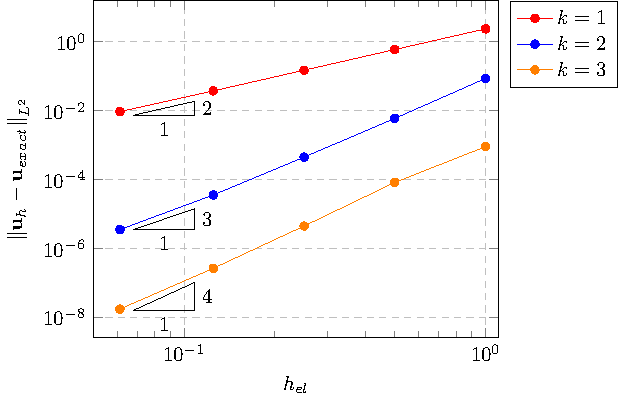
\includegraphics[trim={0cm 0cm 2.0cm 0cm},clip,scale=0.75]{Figures/bishop-disp-03.pdf}} \hfill
%     \subfloat[\label{fig:bishop-convergence-nu-03-b}Pressure]{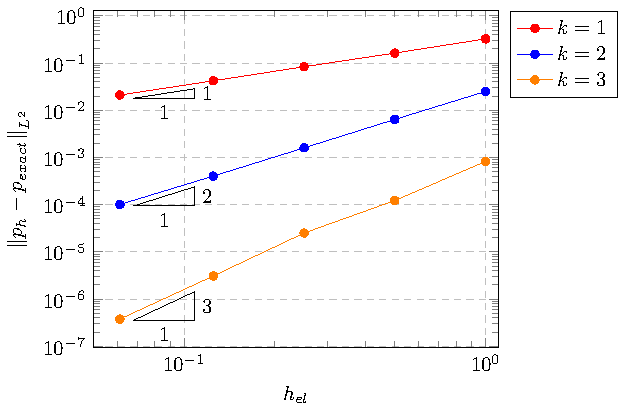
\includegraphics[trim={0cm 0cm 2.0cm 0cm},clip,scale=0.75]{Figures/bishop-pres-03.pdf}}
%     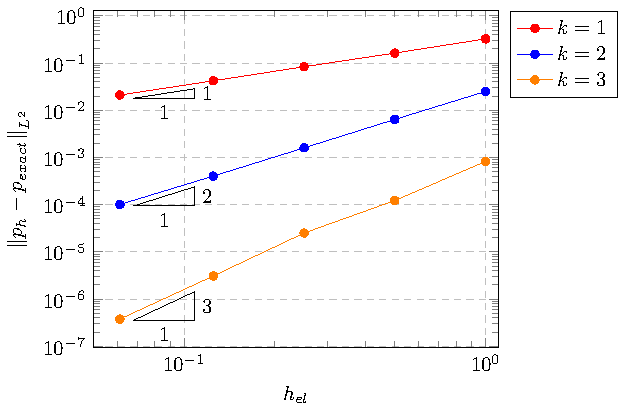
\includegraphics[trim={8.5cm 0cm 0cm 0cm},clip,scale=0.75]{Figures/bishop-pres-03.pdf}
%     \subfloat[\label{fig:bishop-convergence-nu-03-c}Stress]{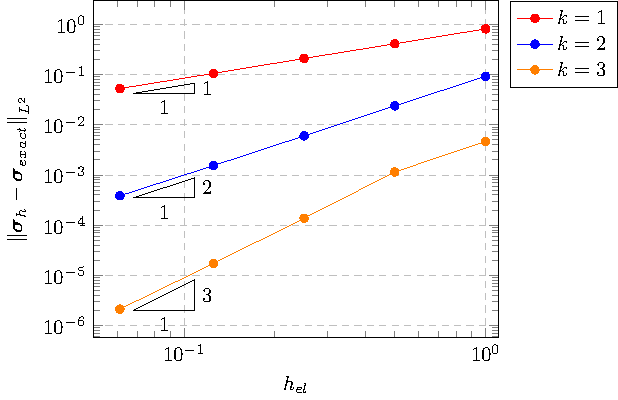
\includegraphics[trim={0cm 0cm 2.0cm 0cm},clip,scale=0.75]{Figures/bishop-stress-03.pdf}} \hfill
%     \subfloat[\label{fig:bishop-convergence-nu-03-d}Divergence]{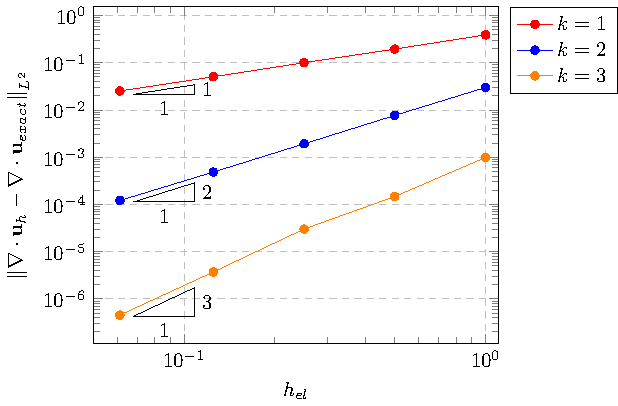
\includegraphics[trim={0cm 0cm 2.0cm 0cm},clip,scale=0.75]{Figures/bishop-div-03.pdf}}
%     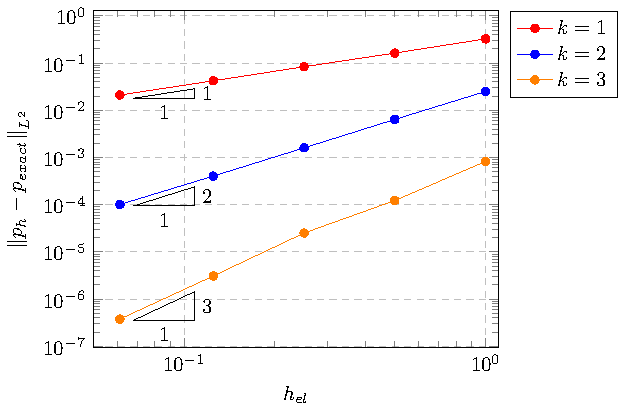
\includegraphics[trim={8.5cm 0cm 0cm 0cm},clip,scale=0.75]{Figures/bishop-pres-03.pdf}
%     \caption{Cantilever beam subjected to an end shear load - convergence analysis for the compressible case ($\nu=0.3$)}
%     \label{fig:bishop-convergence-nu-03}
% \end{figure}

% \begin{figure}
%     \centering
%     \subfloat[\label{fig:bishop-snapshot-a}Displacement]{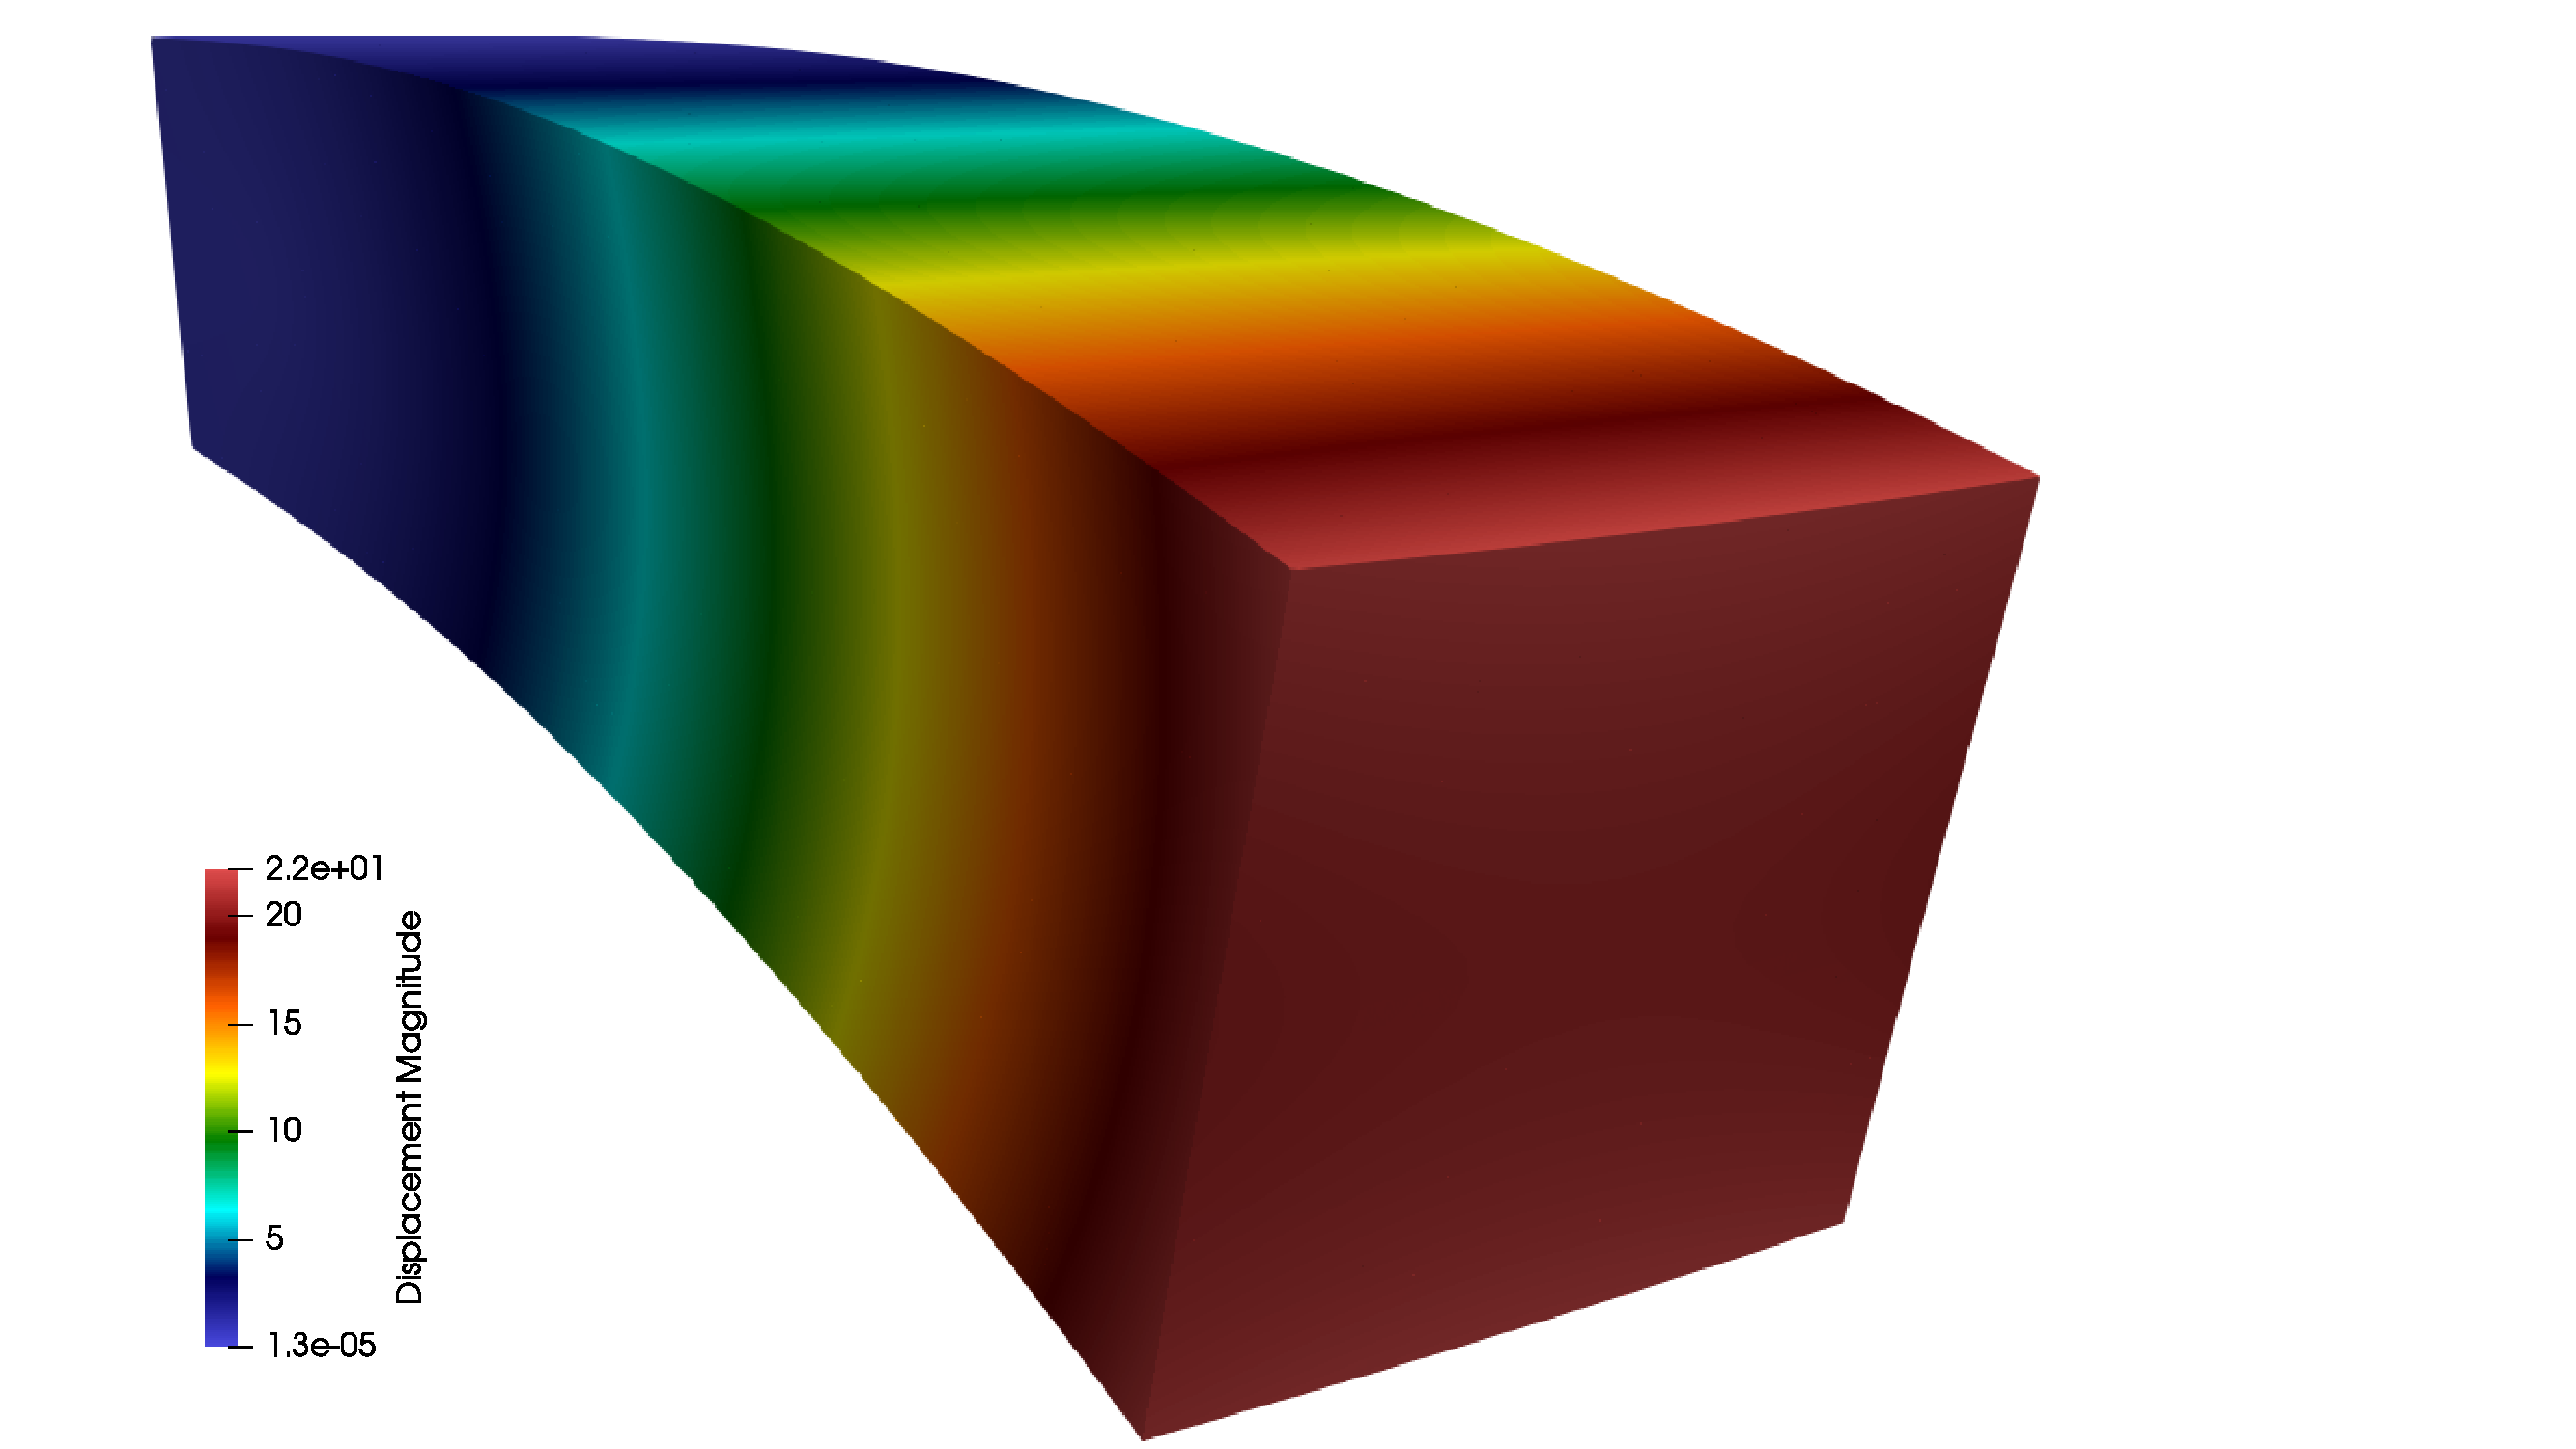
\includegraphics[trim={2.5cm 0cm 9.2cm 0cm},clip,scale=0.2]{Figures/bishop-snapshot-a.pdf}} \hfill
%     \subfloat[\label{fig:bishop-snapshot-b}Pressure]{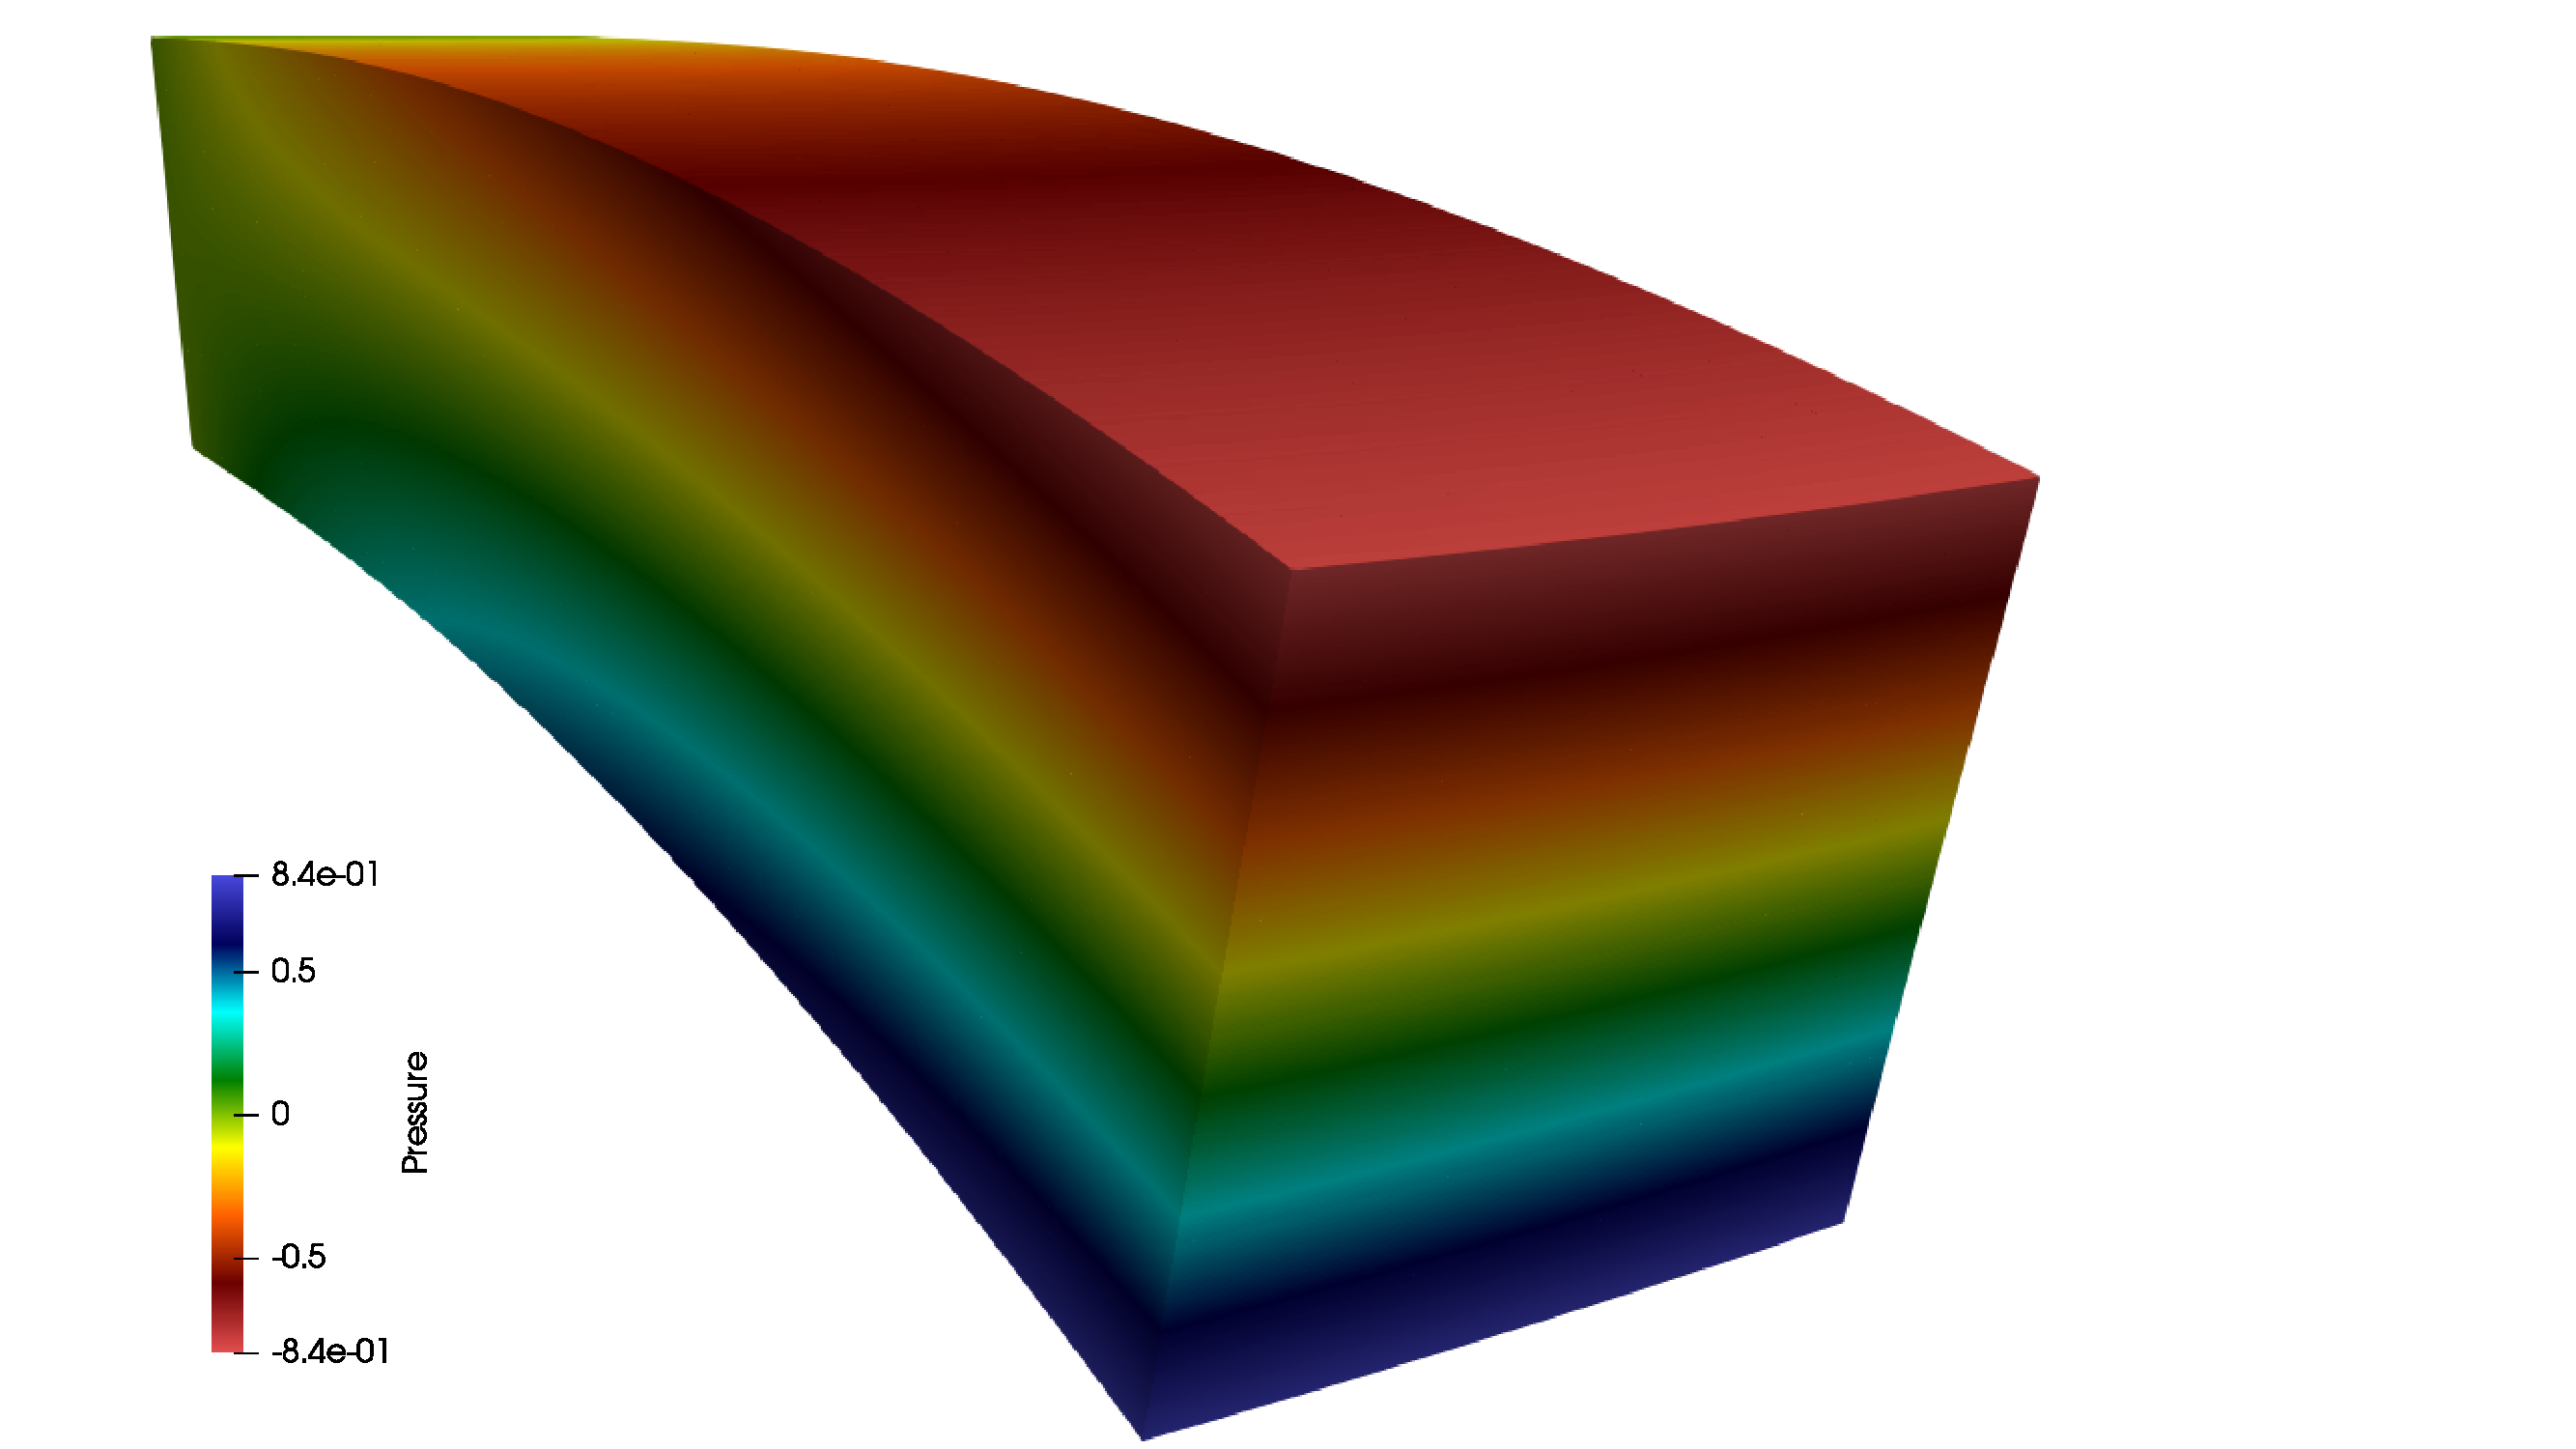
\includegraphics[trim={2.5cm 0cm 9.2cm 0cm},clip,scale=0.2]{Figures/bishop-snapshot-b.pdf}} \\
%     \subfloat[\label{fig:bishop-snapshot-c}Normal stress $\sigma_{zz}$]{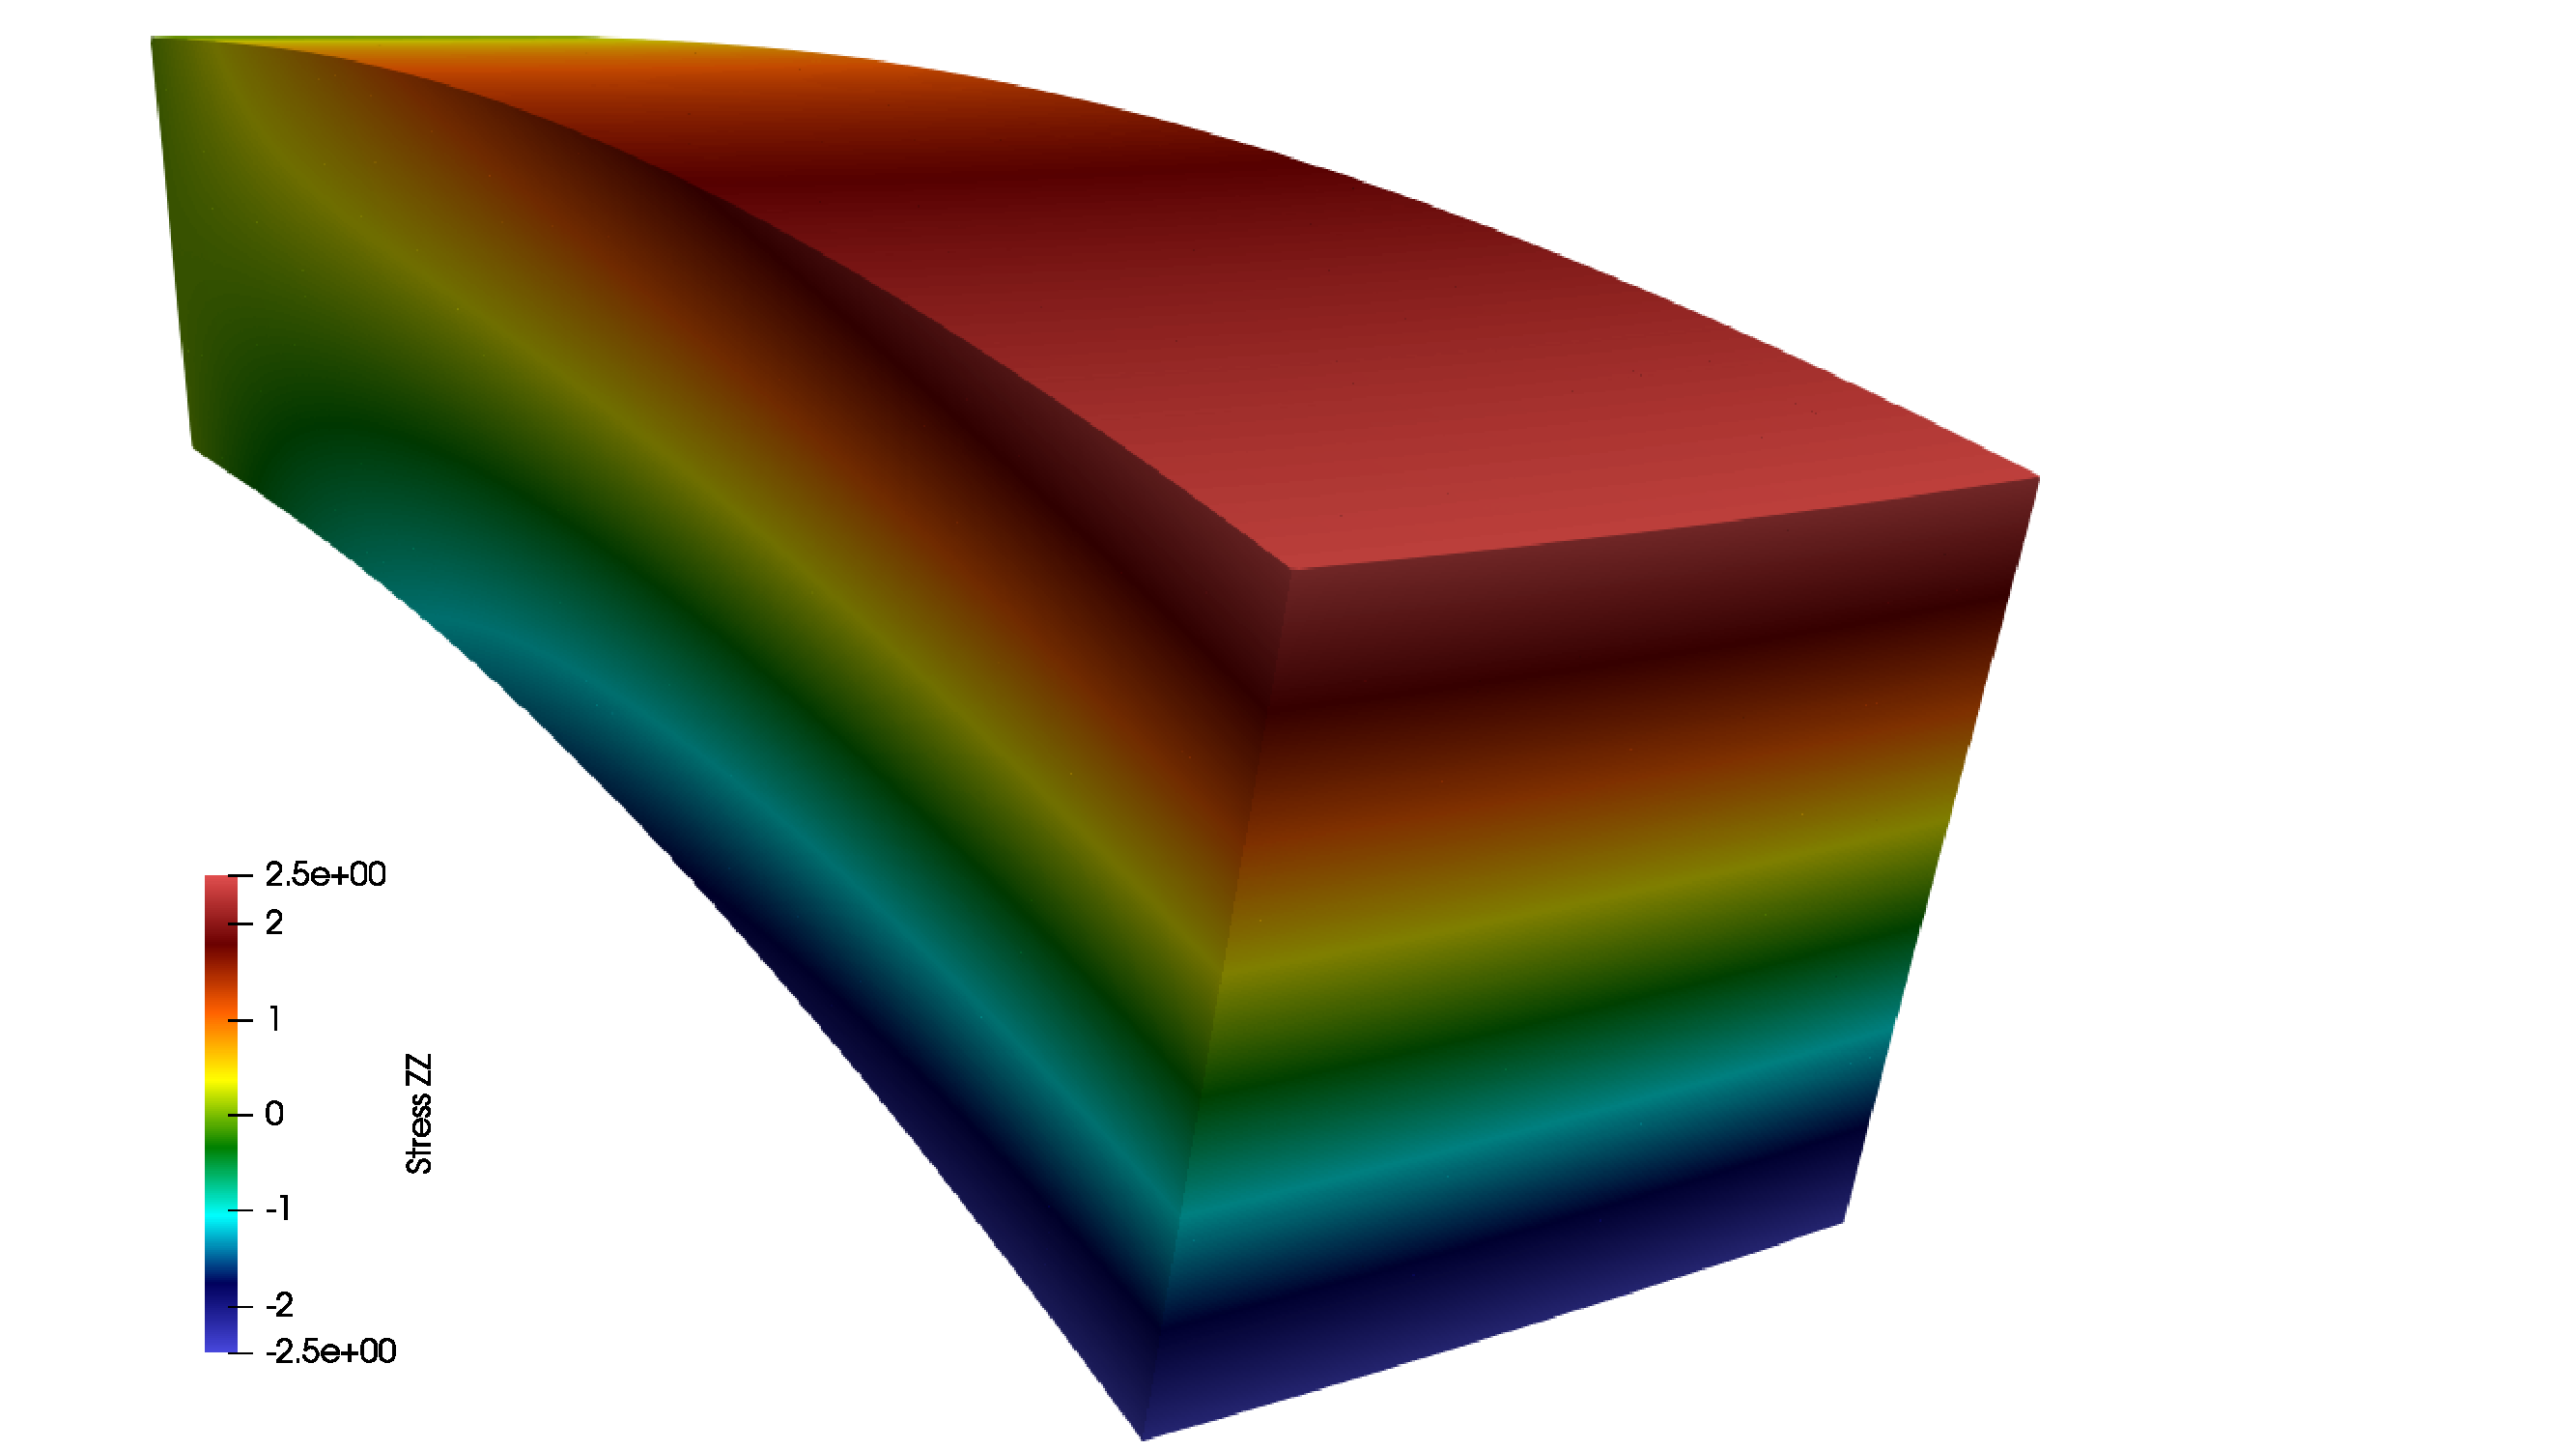
\includegraphics[trim={2.5cm 0cm 9.2cm 0cm},clip,scale=0.2]{Figures/bishop-snapshot-c.pdf}} \hfill
%     \subfloat[\label{fig:bishop-snapshot-d}Shear stress $\sigma_{yz}$]{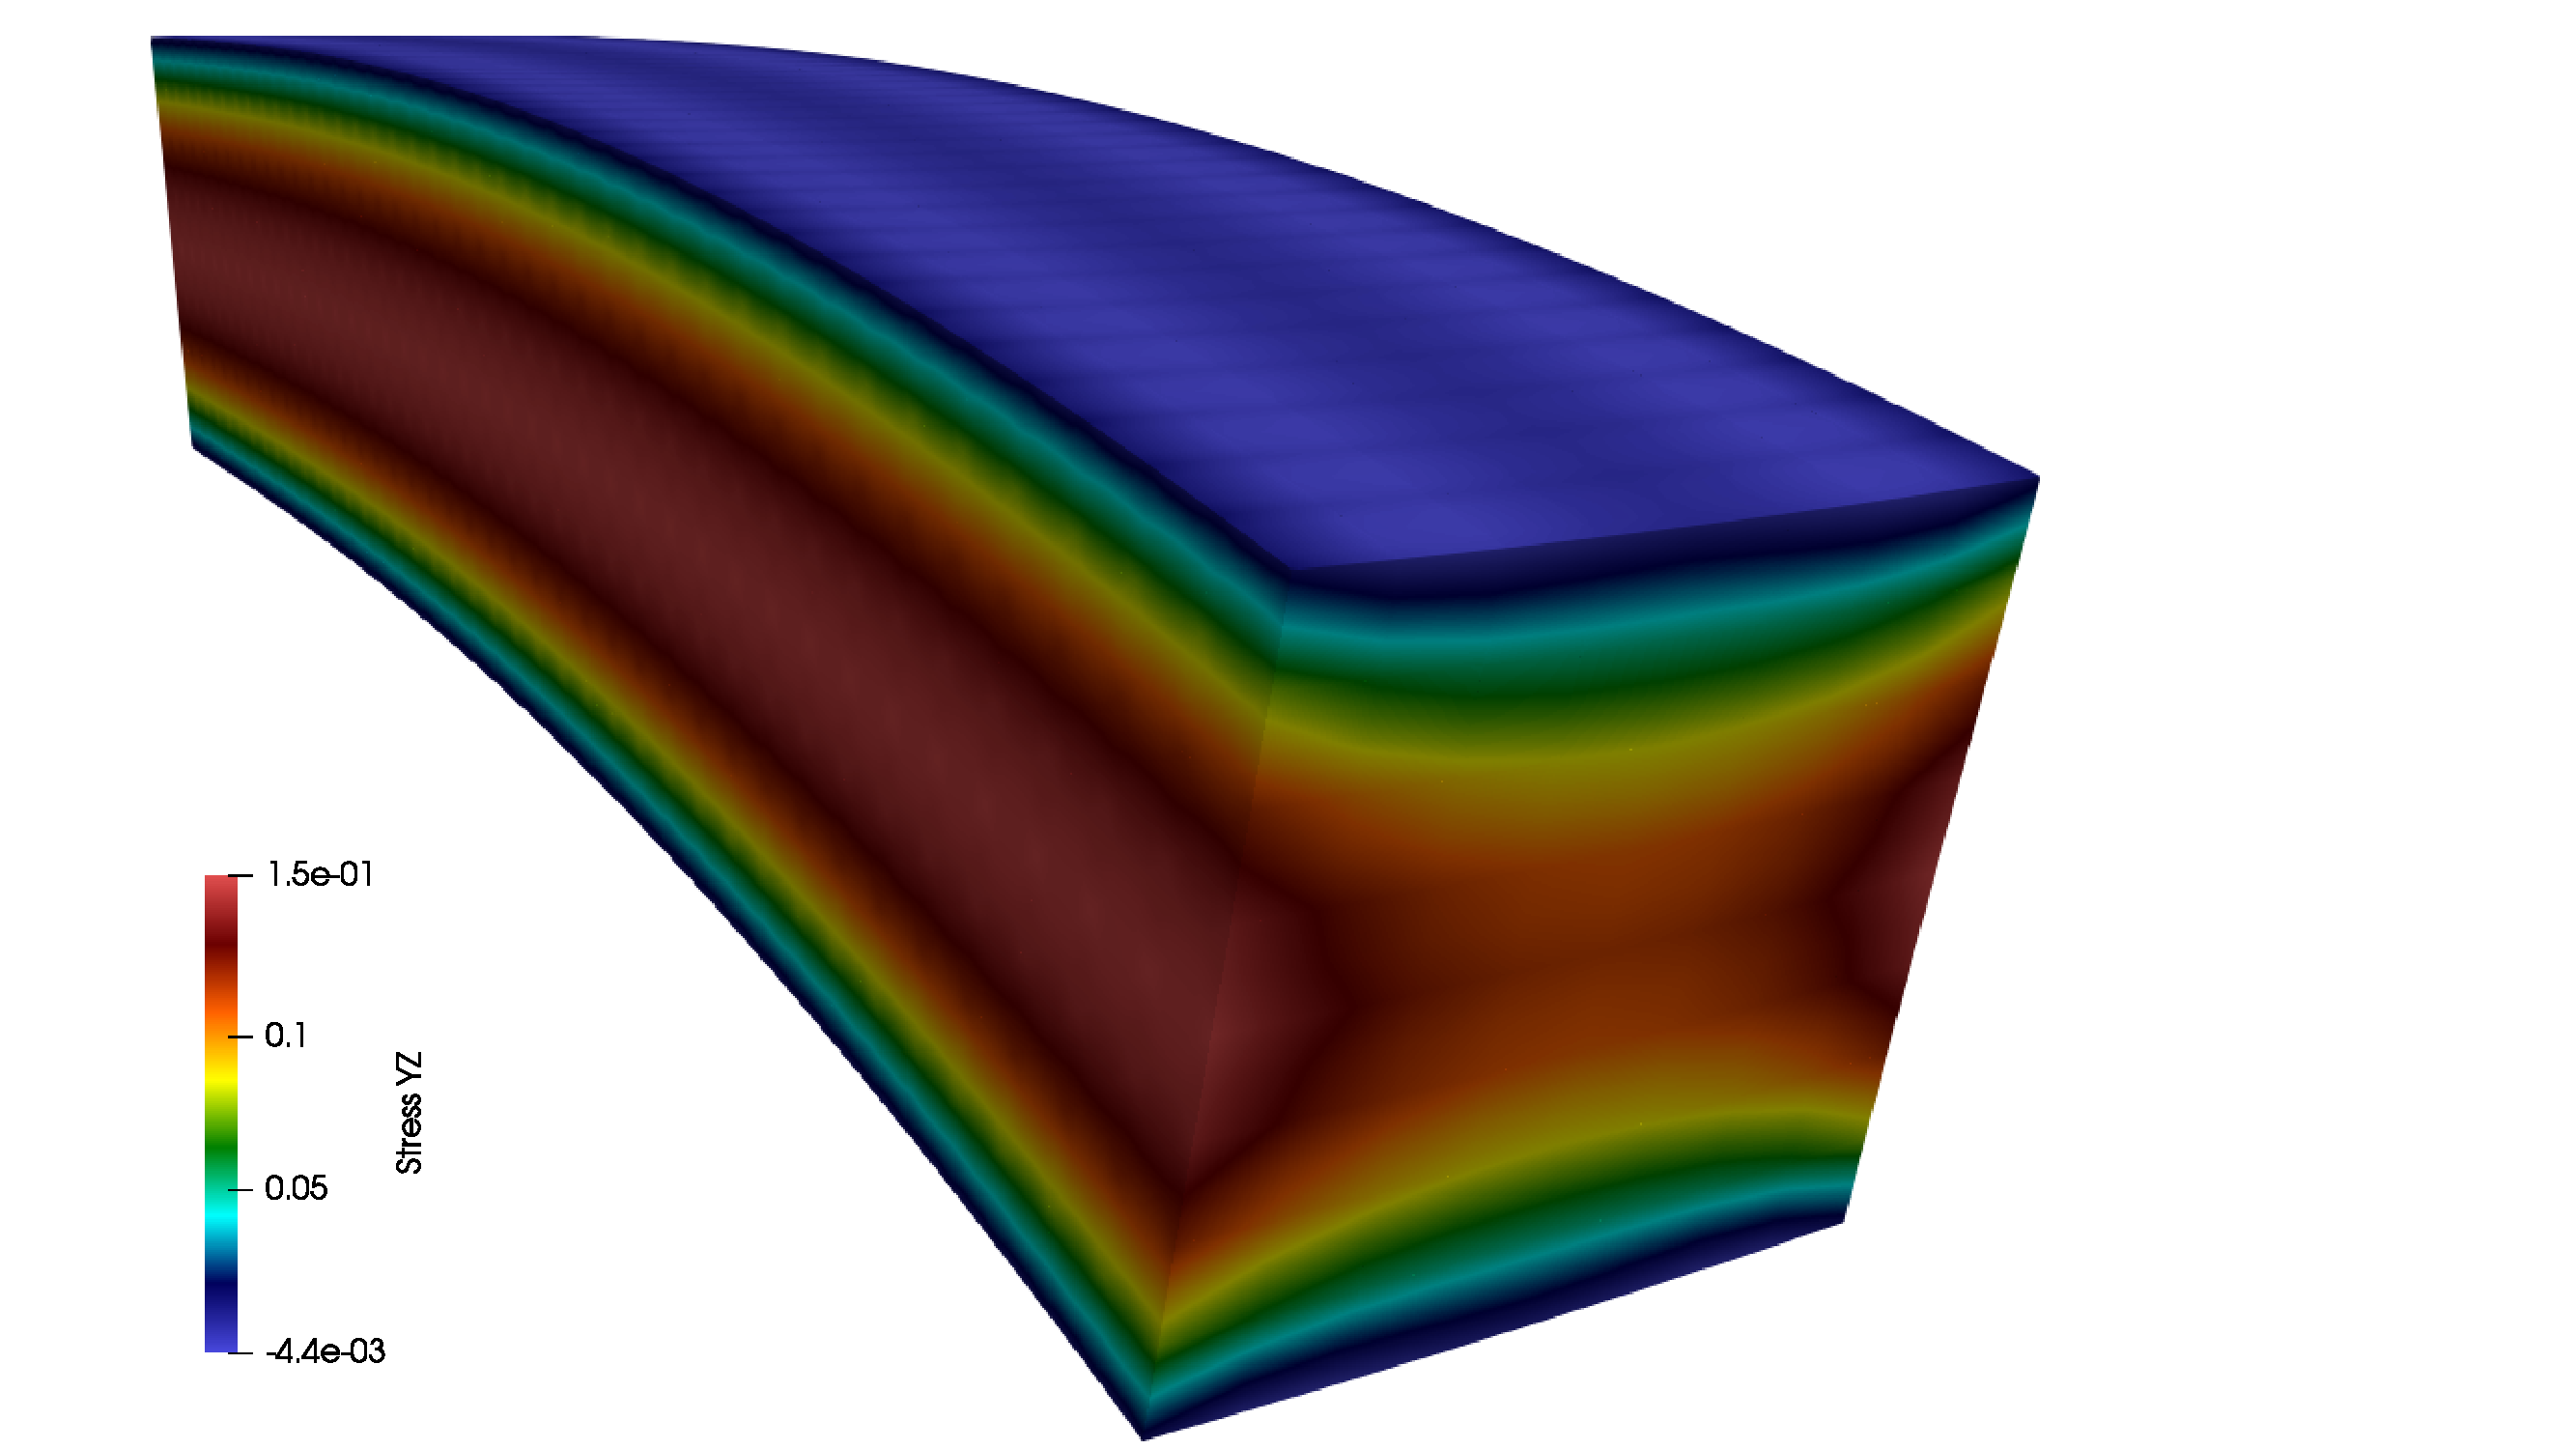
\includegraphics[trim={2.5cm 0cm 9.2cm 0cm},clip,scale=0.2]{Figures/bishop-snapshot-d.pdf}}
%     \caption{Cantilever beam subjected to an end shear load - snapshots for $\nu=0.3$}
%     \label{fig:bishop-snapshot}
% \end{figure}

In order to assess the proposed methodology in different compressibility regimes, the same analysis is performed considering $\nu=0.49$, $\nu=0.4999$, $\nu=0.499999$ and $\nu=0.5$. The convergence results are shown in Figures \ref{fig:bishop-convergence-nu-049}-\ref{fig:bishop-convergence-nu-05}, where optimal convergence rates are achieved independently of the poisson coefficient. This is a nice feature as many formulations present a locking phenomena under quasi and full incompressibility. Also, for the incompressible case ($\nu=0.5$), a divergence free displacement field is obtained even for the coarsest mesh, with the error bounded to the machine precision.

% \begin{figure}
%     \centering
%     \subfloat[\label{fig:bishop-convergence-nu-049-a}Displacement]{\includegraphics[trim={0cm 0cm 2.0cm 0cm},clip,scale=0.75]{Figures/bishop-disp-049.pdf}} \hfill
%     \subfloat[\label{fig:bishop-convergence-nu-049-b}Pressure]{\includegraphics[trim={0cm 0cm 2.0cm 0cm},clip,scale=0.75]{Figures/bishop-pres-049.pdf}}
%     \includegraphics[trim={8.5cm 0cm 0cm 0cm},clip,scale=0.75]{Figures/bishop-pres-049.pdf}
%     \subfloat[\label{fig:bishop-convergence-nu-049-c}Stress]{\includegraphics[trim={0cm 0cm 2.0cm 0cm},clip,scale=0.75]{Figures/bishop-stress-049.pdf}} \hfill
%     \subfloat[\label{fig:bishop-convergence-nu-049-d}Divergence]{\includegraphics[trim={0cm 0cm 2.0cm 0cm},clip,scale=0.75]{Figures/bishop-div-049.pdf}}
%     \includegraphics[trim={8.5cm 0cm 0cm 0cm},clip,scale=0.75]{Figures/bishop-pres-049.pdf}
%     \caption{Cantilever beam subjected to an end shear load - convergence analysis for the compressible case ($\nu=0.49$)}
%     \label{fig:bishop-convergence-nu-049}
% \end{figure}
% \begin{figure}
%     \centering
%     \subfloat[\label{fig:bishop-convergence-nu-04999-a}Displacement]{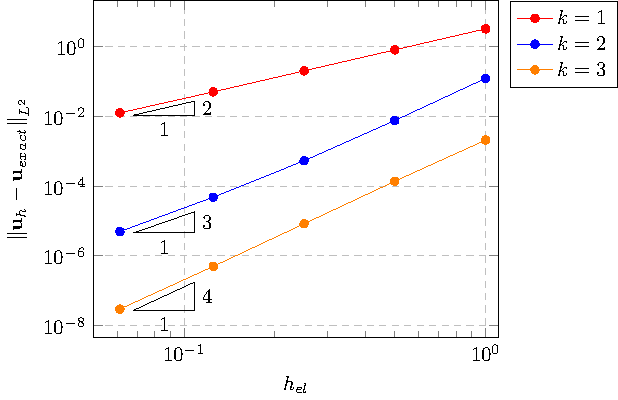
\includegraphics[trim={0cm 0cm 2.0cm 0cm},clip,scale=0.75]{Figures/bishop-disp-04999.pdf}} \hfill
%     \subfloat[\label{fig:bishop-convergence-nu-04999-b}Pressure]{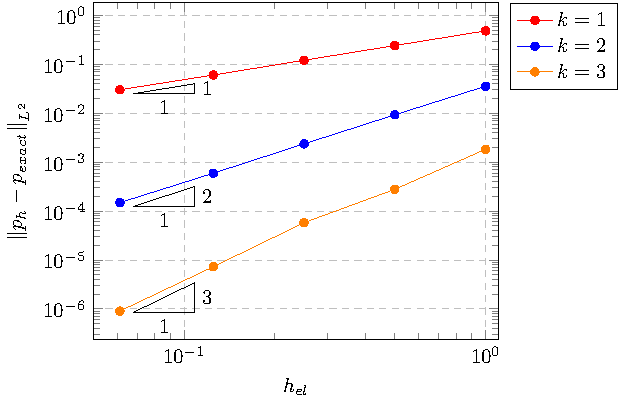
\includegraphics[trim={0cm 0cm 2.0cm 0cm},clip,scale=0.75]{Figures/bishop-pres-04999.pdf}}
%     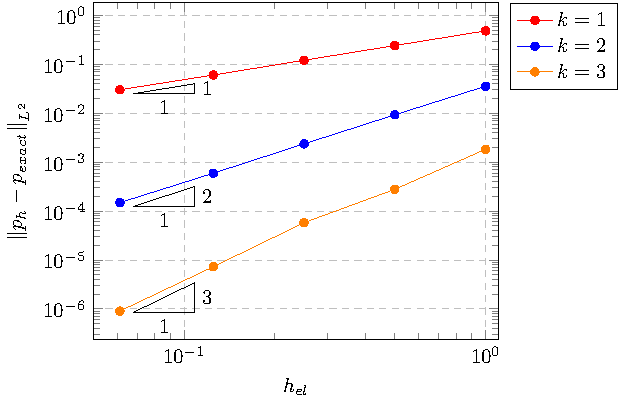
\includegraphics[trim={8.5cm 0cm 0cm 0cm},clip,scale=0.75]{Figures/bishop-pres-04999.pdf}
%     \subfloat[\label{fig:bishop-convergence-nu-04999-c}Stress]{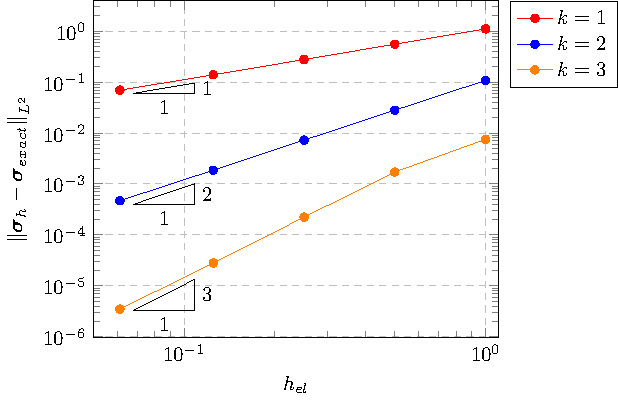
\includegraphics[trim={0cm 0cm 2.0cm 0cm},clip,scale=0.75]{Figures/bishop-stress-04999.pdf}} \hfill
%     \subfloat[\label{fig:bishop-convergence-nu-04999-d}Divergence]{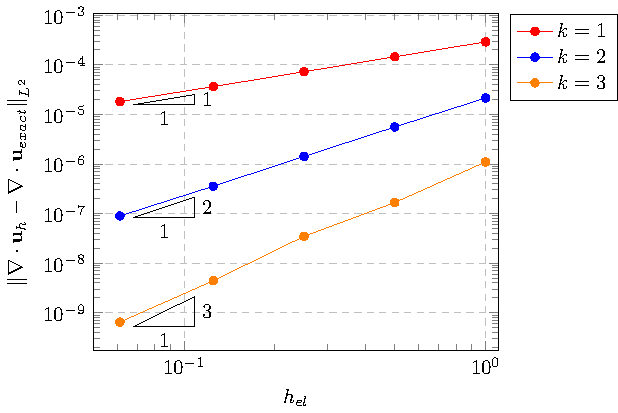
\includegraphics[trim={0cm 0cm 2.0cm 0cm},clip,scale=0.75]{Figures/bishop-div-04999.pdf}}
%     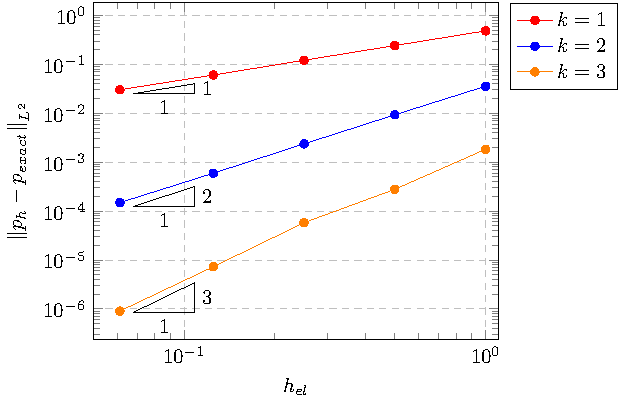
\includegraphics[trim={8.5cm 0cm 0cm 0cm},clip,scale=0.75]{Figures/bishop-pres-04999.pdf}
%     \caption{Cantilever beam subjected to an end shear load - convergence analysis for the quasi-incompressible case ($\nu=0.4999$)}
%     \label{fig:bishop-convergence-nu-04999}
% \end{figure}
% \begin{figure}
%     \centering
%     \subfloat[\label{fig:bishop-convergence-nu-0499999-a}Displacement]{\includegraphics[trim={0cm 0cm 2.0cm 0cm},clip,scale=0.75]{Figures/bishop-disp-0499999.pdf}} \hfill
%     \subfloat[\label{fig:bishop-convergence-nu-0499999-b}Pressure]{\includegraphics[trim={0cm 0cm 2.0cm 0cm},clip,scale=0.75]{Figures/bishop-pres-0499999.pdf}}
%     \includegraphics[trim={8.5cm 0cm 0cm 0cm},clip,scale=0.75]{Figures/bishop-pres-0499999.pdf}
%     \subfloat[\label{fig:bishop-convergence-nu-0499999-c}Stress]{\includegraphics[trim={0cm 0cm 2.0cm 0cm},clip,scale=0.75]{Figures/bishop-stress-0499999.pdf}} \hfill
%     \subfloat[\label{fig:bishop-convergence-nu-0499999-d}Divergence]{\includegraphics[trim={0cm 0cm 2.0cm 0cm},clip,scale=0.75]{Figures/bishop-div-0499999.pdf}}
%     \includegraphics[trim={8.5cm 0cm 0cm 0cm},clip,scale=0.75]{Figures/bishop-pres-0499999.pdf}
%     \caption{Cantilever beam subjected to an end shear load - convergence analysis for the quasi-incompressible case ($\nu=0.499999$)}
%     \label{fig:bishop-convergence-nu-0499999}
% \end{figure}
% \begin{figure}
%     \centering
%     \subfloat[\label{fig:bishop-convergence-nu-05-a}Displacement]{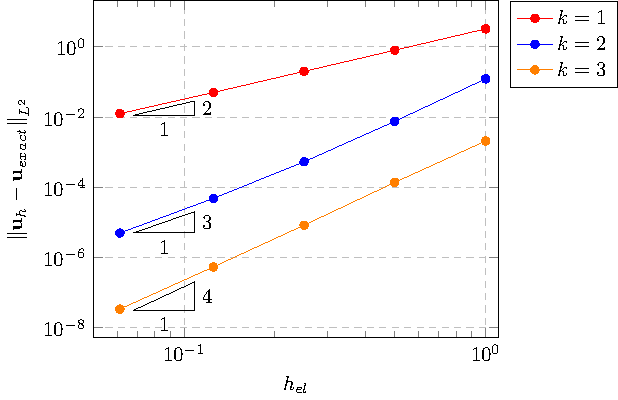
\includegraphics[trim={0cm 0cm 2.0cm 0cm},clip,scale=0.75]{Figures/bishop-disp-05.pdf}} \hfill
%     \subfloat[\label{fig:bishop-convergence-nu-05-b}Pressure]{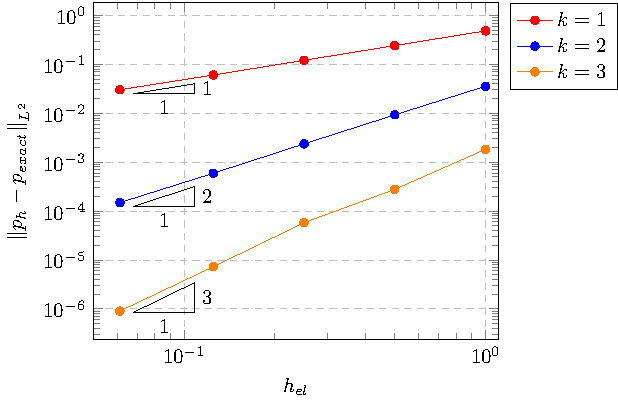
\includegraphics[trim={0cm 0cm 2.0cm 0cm},clip,scale=0.75]{Figures/bishop-pres-05.pdf}}
%     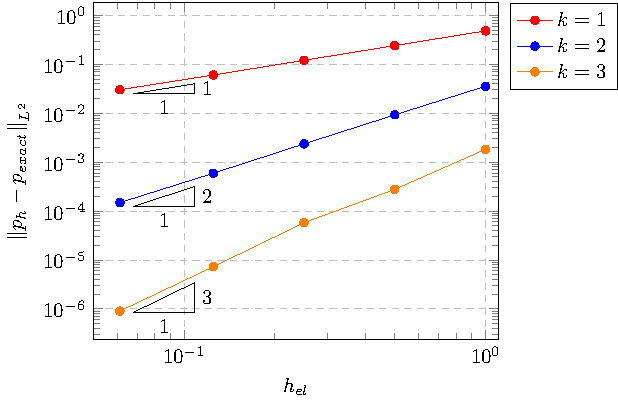
\includegraphics[trim={8.5cm 0cm 0cm 0cm},clip,scale=0.75]{Figures/bishop-pres-05.pdf}
%     \subfloat[\label{fig:bishop-convergence-nu-05-c}Stress]{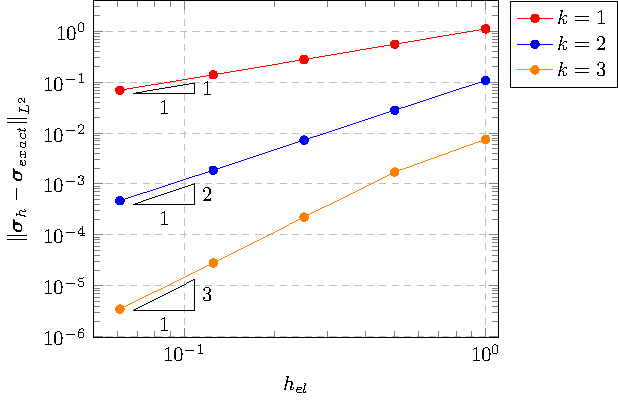
\includegraphics[trim={0cm 0cm 2.0cm 0cm},clip,scale=0.75]{Figures/bishop-stress-05.pdf}} \hfill
%     \subfloat[\label{fig:bishop-convergence-nu-05-d}Divergence]{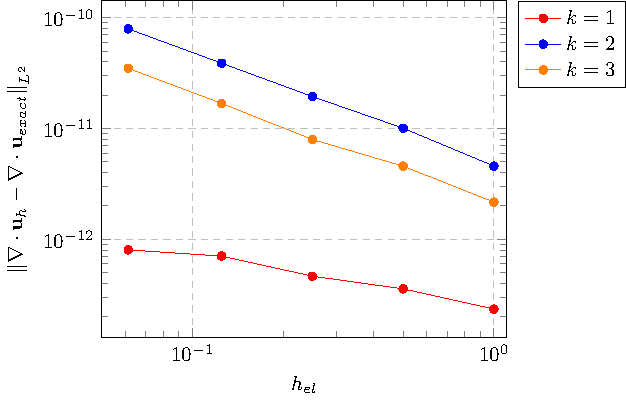
\includegraphics[trim={0cm 0cm 2.0cm 0cm},clip,scale=0.75]{Figures/bishop-div-05.pdf}}
%     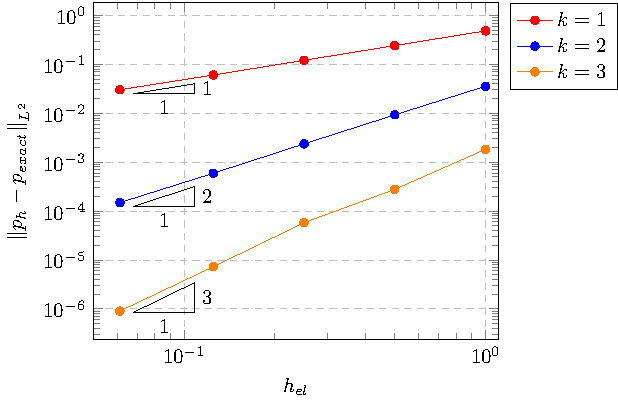
\includegraphics[trim={8.5cm 0cm 0cm 0cm},clip,scale=0.75]{Figures/bishop-pres-05.pdf}
%     \caption{Cantilever beam subjected to an end shear load - convergence analysis for the incompressible case ($\nu=0.5$)}
%     \label{fig:bishop-convergence-nu-05}
% \end{figure}

\subsection{Cook's membrane \label{subsec:cook}}

The Cook's membrane is a classical benchmark for the study of locking phenomena of incompressible or nearly-incompressible elasticity problems under shear and bending conditions. It consists of a tapered cantilever beam clamped at its left side and subjected to a shear load in the $y$ direction at $x=48$ mm equal to $F=6.25$ N/mm, according to Figure \ref{fig:cooks-geometry}. The material is assumed to have a linear behaviour with a constant Young modulus $E=240.565$ MPa and two different Poisson coefficients were tested according to the references: $\nu=0.4999$ and $\nu=0.4999999$. This problem can be seen in many books and papers, such as in \cite{cook1989concepts,elguedj2008b,cesar1999new}, with different material properties, geometries and boundary conditions. Some works also studied this problem in the regime of large displacements and strains, under elastic and elastoplastic materials \cite{chavan2007locking,elguedj2008b,de1996design}. In this work, we only focus on the linear elastic analysis.

\begin{figure}[H]
    \centering
    \input{cooks-membrane.pdf_tex}
    \caption{Cook's membrane. Geometry.}
    \label{fig:cooks-geometry}
\end{figure}

At first, we perform plane strain analyses using structured meshes with triangular and quadrilateral partitions with uniform refinements, so that the number of elements per edge is given by $N_e=2^n$, with $n={0,1,2,3,4,5}$. Some of the meshes employed are depicted in Figures \ref{fig:cooks-2d-tri-meshes}-\ref{fig:cooks-2d-quad-meshes}.

\begin{figure}[H]
	\centering
	\subfloat[$N_e=1$]{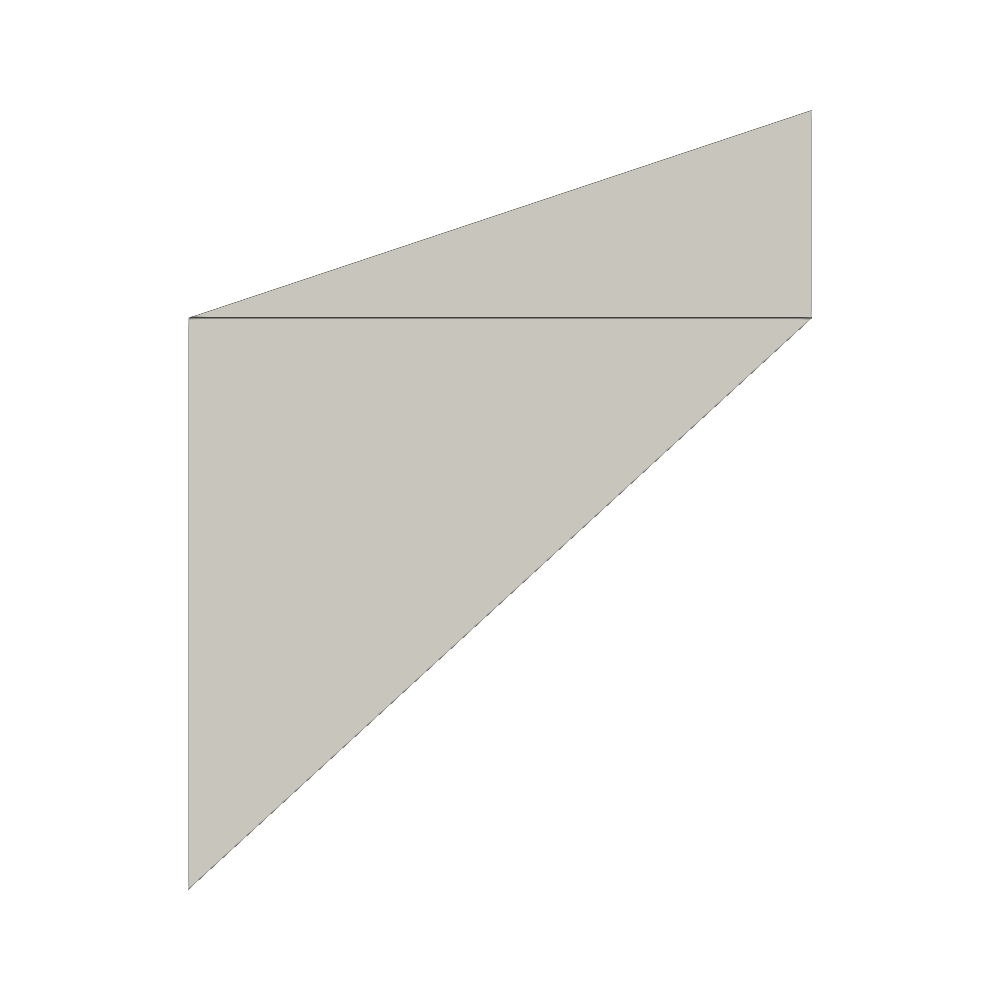
\includegraphics[width=0.25\textwidth, trim={4cm 4cm 4cm 3.5cm}, clip]{cooks-2d-tri-mesh-1.png}}
	\subfloat[$N_e=2$]{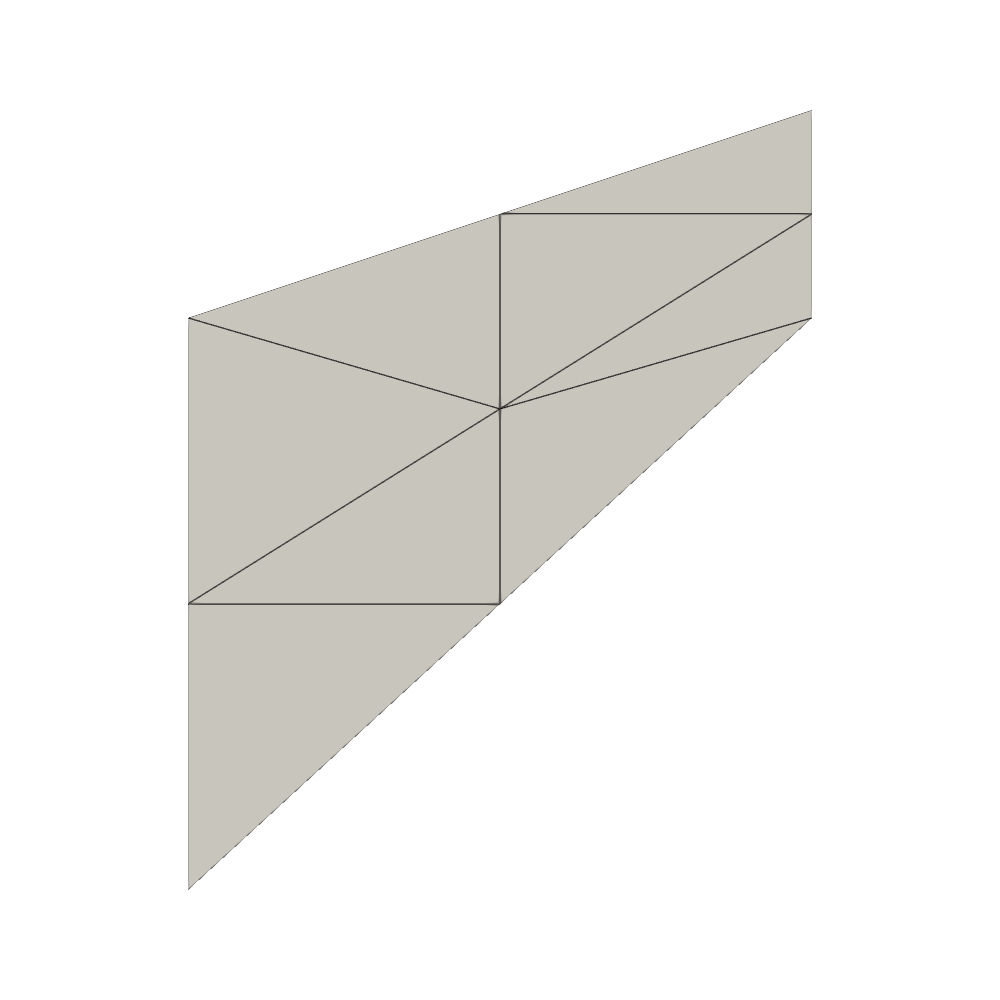
\includegraphics[width=0.25\textwidth, trim={4cm 4cm 4cm 3.5cm}, clip]{cooks-2d-tri-mesh-2.png}}
	\subfloat[$N_e=8$]{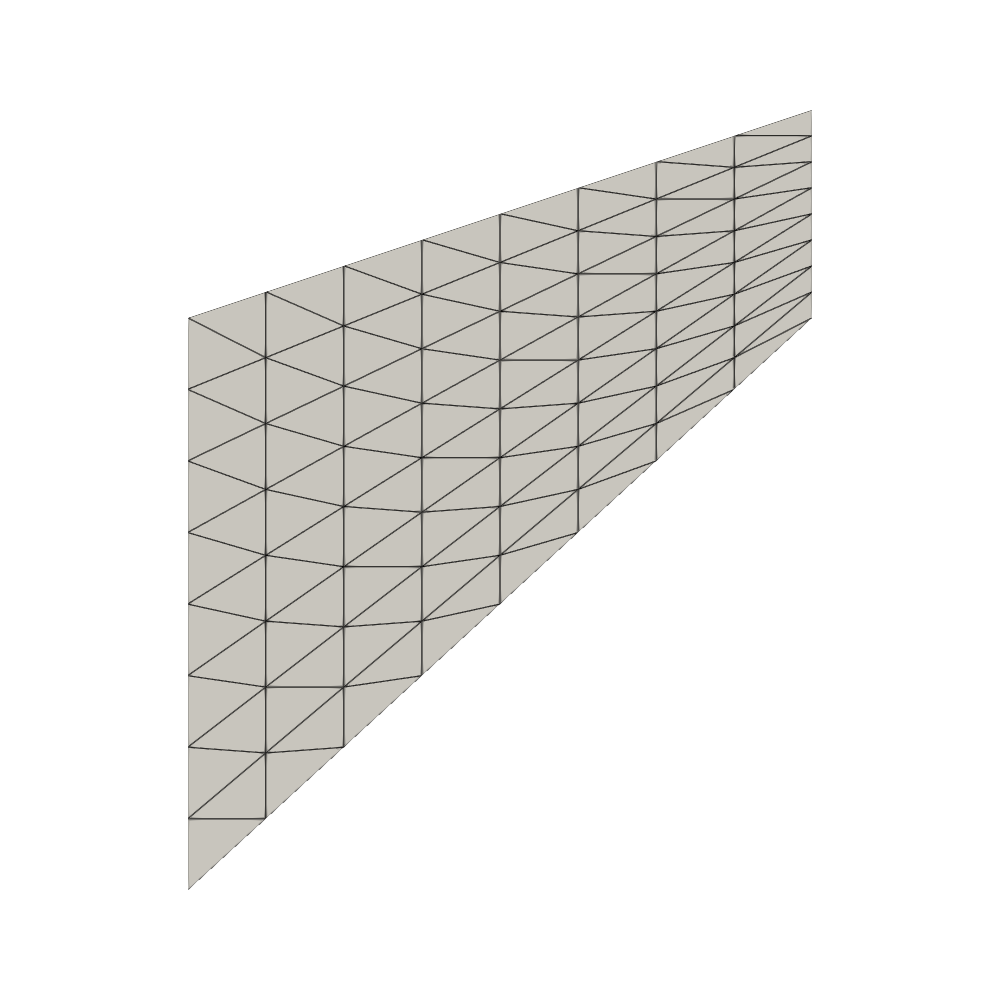
\includegraphics[width=0.25\textwidth, trim={4cm 4cm 4cm 3.5cm}, clip]{cooks-2d-tri-mesh-8.png}}
	\subfloat[$N_e=32$]{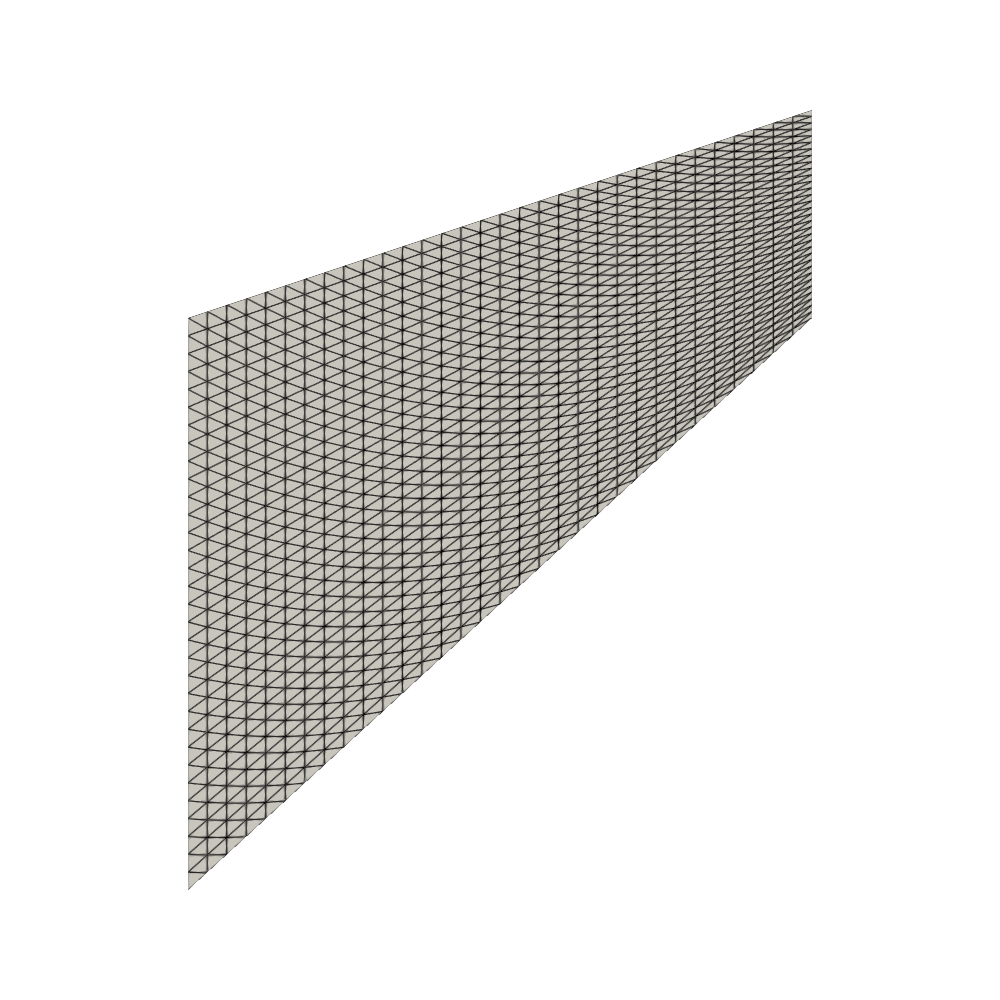
\includegraphics[width=0.25\textwidth, trim={4cm 4cm 4cm 3.5cm}, clip]{cooks-2d-tri-mesh-32.png}}
	\caption{Cook's membrane. Plane strain meshes with triangular partitions.}
	\label{fig:cooks-2d-tri-meshes}
\end{figure}

\begin{figure}[H]
	\centering
	\subfloat[$N_e=1$]{
\includegraphics[width=0.25\textwidth, trim={4cm 4cm 4cm 3.5cm}, clip]{cooks-2d-quad-mesh-1.png}} \hfill
	\subfloat[$N_e=2$]{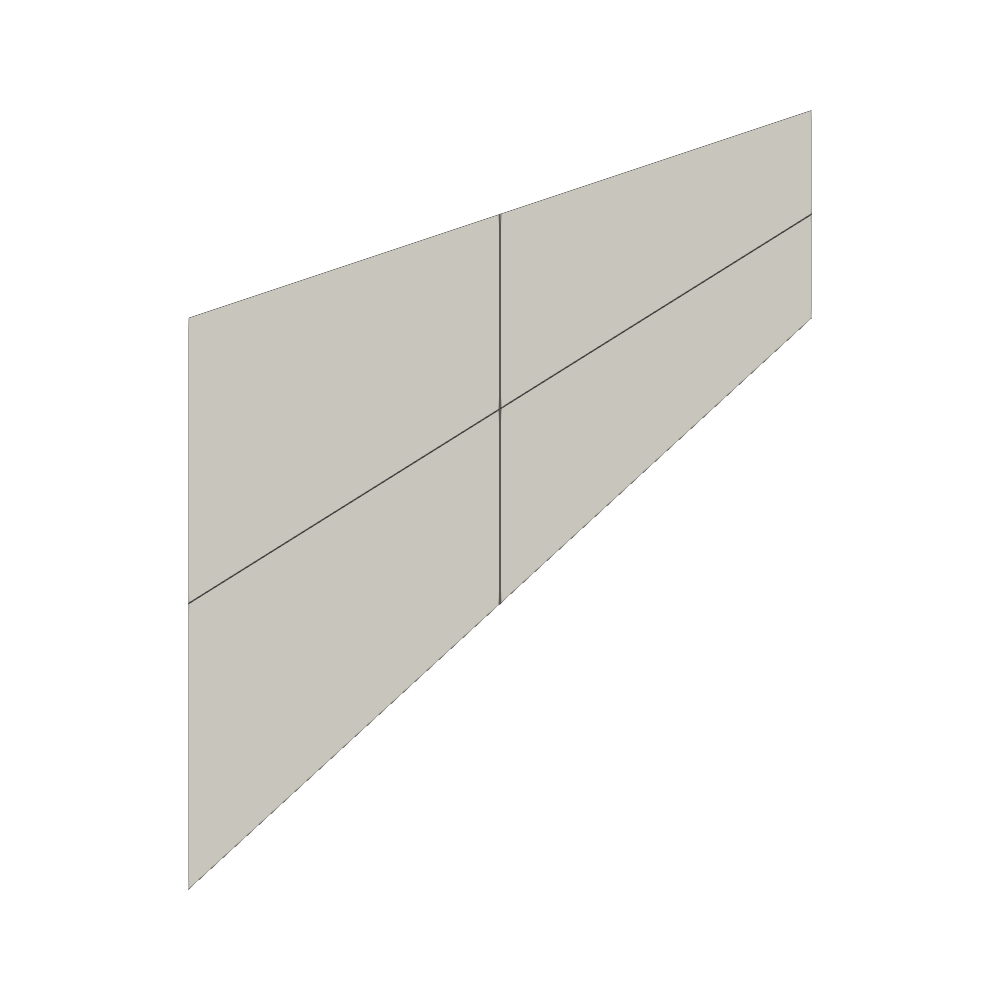
\includegraphics[width=0.25\textwidth, trim={4cm 4cm 4cm 3.5cm}, clip]{cooks-2d-quad-mesh-2.png}} \hfill
	\subfloat[$N_e=8$]{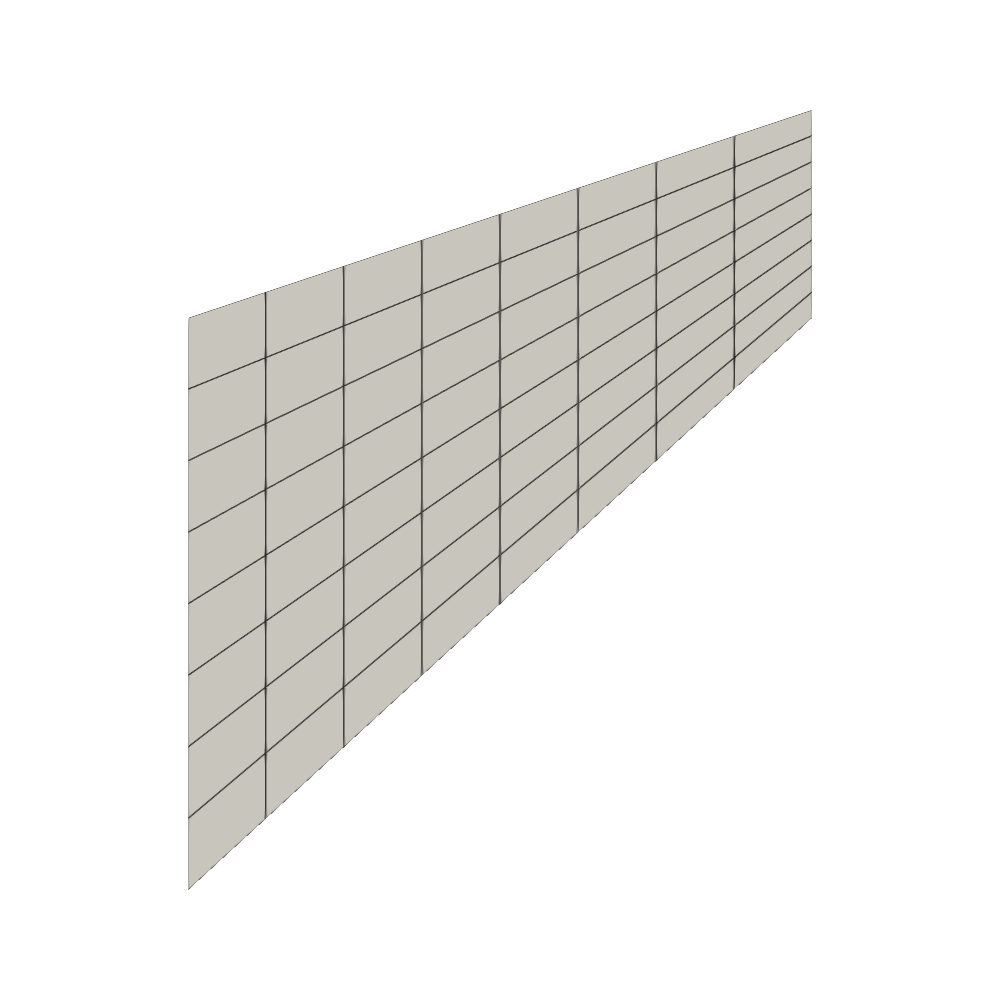
\includegraphics[width=0.25\textwidth, trim={4cm 4cm 4cm 3.5cm}, clip]{cooks-2d-quad-mesh-8.png}} \hfill
	\subfloat[$N_e=32$]{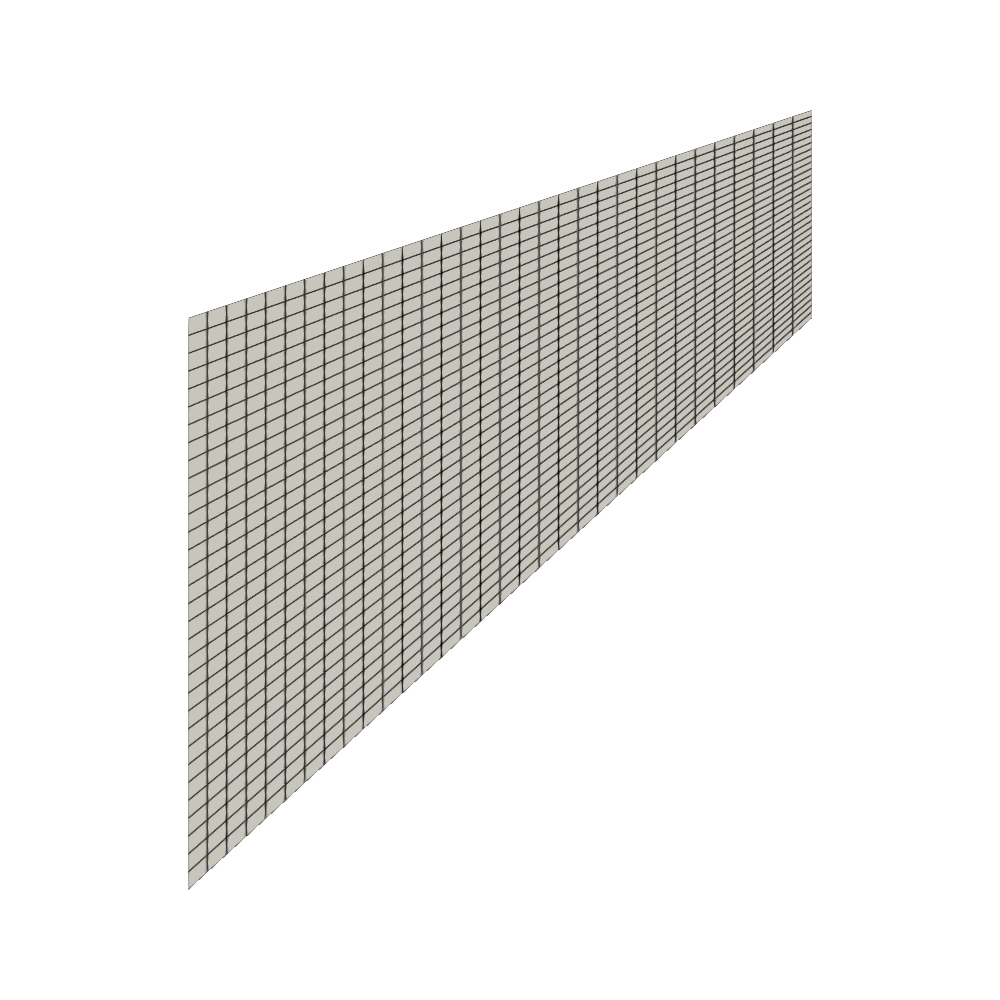
\includegraphics[width=0.25\textwidth, trim={4cm 4cm 4cm 3.5cm}, clip]{cooks-2d-quad-mesh-32.png}}
	\caption{Cook's membrane. Plane strain meshes with quadrilateral partitions.}
	\label{fig:cooks-2d-quad-meshes}
\end{figure}

Figure \ref{fig:cooks-2d-displacement} shows a comparison of the vertical displacement of point A for two values of $\nu$ with some numerical results available in the literature \cite{elguedj2008b,cesar1999new} and results obtained with classical $\mathcal{Q}^1$ and $\mathcal{T}^1$ quadrilateral and triangular elements, respectively, with $H^1$ functions. One notices that our approach leads to a locking-free solution and converges to the reference solutions, while the solutions obtained with classical $H^1$ shape-functions clearly exhibit an excessive bending stiffness leading to a wrong representation of the problem's cinematic.

\begin{figure}[H]
	\centering
	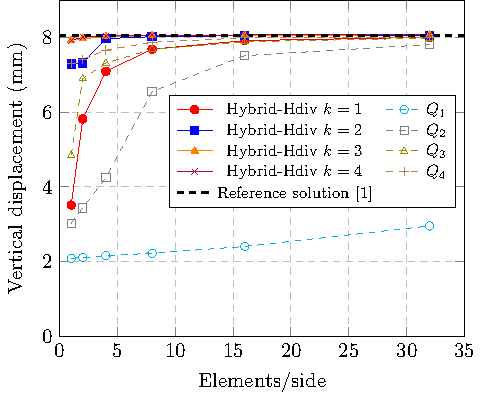
\includegraphics[scale=1.0]{cook-2d-disp-0.4999}
	\caption{Cook's membrane. Vertical displacement of point A.}
	\label{fig:cooks-2d-displacement}
\end{figure}

\subsection{Application problem\label{subsec:module}}

With the objective of testing the method's robustness regarding complex geometries, the proposed methodology is applied to a real-world problem. The geometry of a structural hull is depicted in Figure \ref{fig:module-geometry}, with dimensions $L=1\m$, $r_i=0.345\m$, $r_e=0.390\m$. The hull is subjected to an internal pressure of $p=10.34$ MPa and fixed in the normal direction of all other faces. The material is assumed to have a linear behaviour with a constant Young modulus $E=210000$ MPa and Poisson coefficient $\nu=0.3$. Since the problem is axisymmetric, only one-forth of the domain is modeled, as shown in Figure \ref{fig:module-geometry}. The results obtained with the proposed formulation are compared with the results obtained using the classical Taylor-Hood formulation.

\begin{figure}[h]
    \centering
    \def\svgwidth{450pt} 
    % 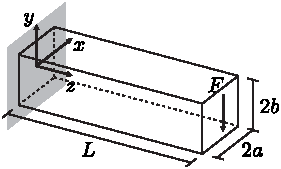
\includegraphics{bishop-beam-geometry.pdf}
    \input{hull-domain.pdf_tex}
    % 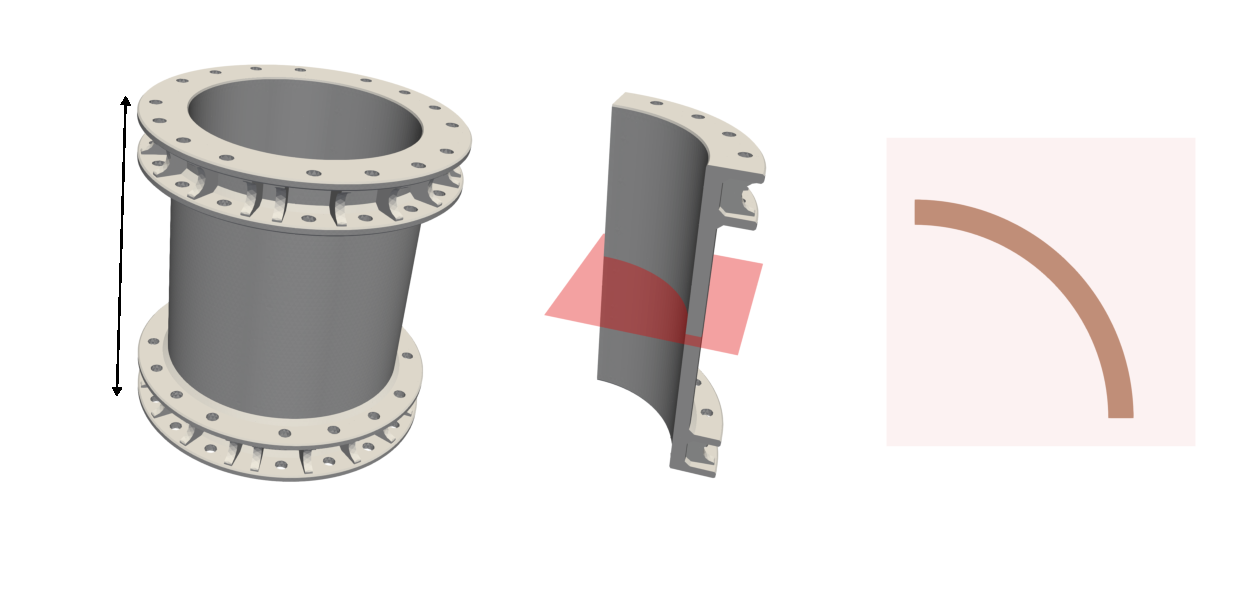
\includegraphics{hull-domain.pdf}
    \caption{Geometry of the structural hull. Only one-forth of the domain is modeled due to axisymmetry of the domain.}
    \label{fig:module-geometry}
\end{figure}

The problem is solved using an unstructured tetrahedral mesh with 68,258 elements, as shown in Figure \ref{fig:module-mesh}. Both the proposed Hybrid-Hdiv and the Taylor-Hood formulations are tested with polynomial degrees $k=2$ and $k=3$, resulting in four different simulations. The results are compared in terms of displacement magnitude, pressure, and Von Mises stresses along a line defined by the points $(259.86, 259.86, 0)$ mm and $(259.86, 259.86, 1000)$ mm. 

The number of degrees of freedom  for the Hybrid-Hdiv formulation is 1,336,260 for $k=2$ and 2,440,900 for $k=3$. For the Taylor-Hood formulation, the number of DOF is 322,447 for $k=2$ and 1,060,639 for $k=3$. The high number of degrees of freedom when using the Hybrid-Hdiv formulation in this problem is due to the use of tetrahedral elements, which increase the number of faces in the mesh. In the Hybrid-Hdiv method, the number of degrees of freedom is significantly influenced by the number of element faces in the mesh.

\begin{figure}[h]
	\centering
	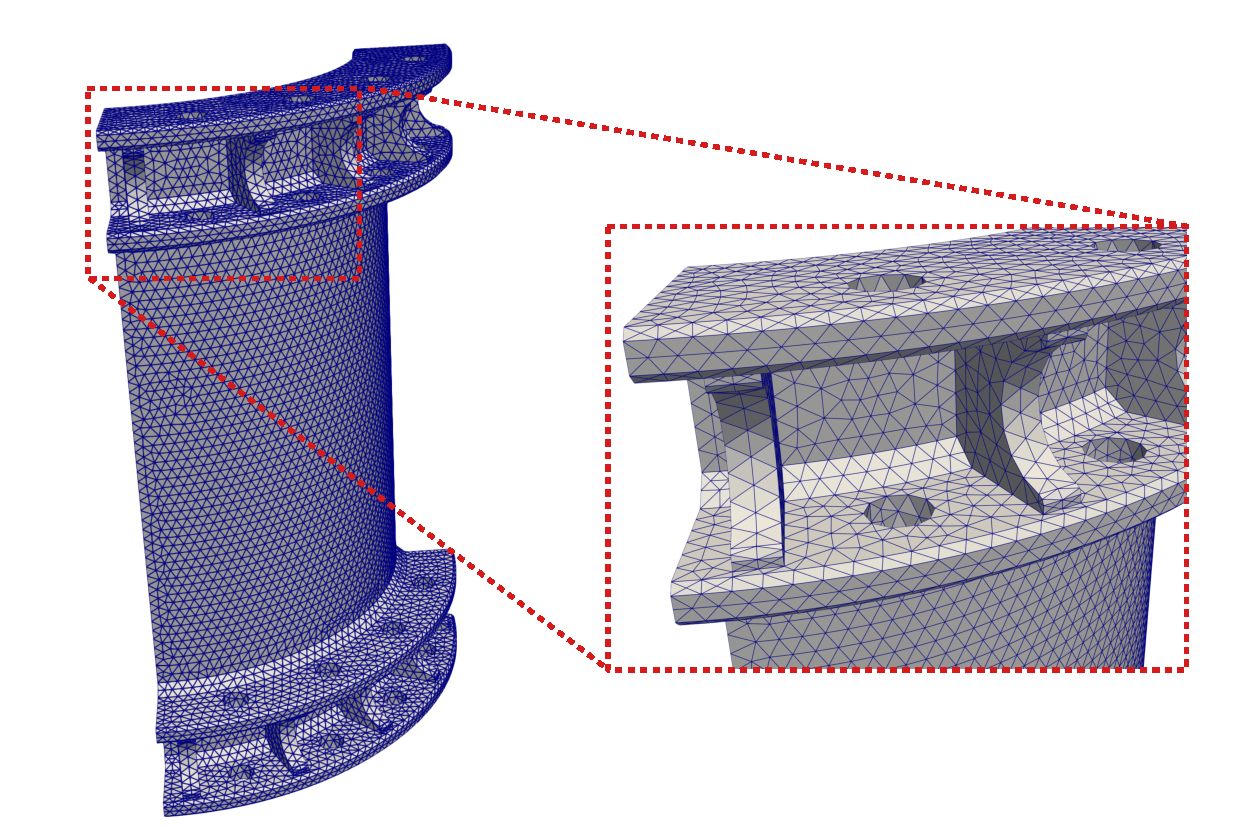
\includegraphics[scale=0.75]{hull-mesh.pdf}
	\caption{Adopted finite element mesh of the hull with zoom in showing the details of the top region of the domain.}
	\label{fig:module-mesh}
\end{figure}

The results for the displacement magnitude, pressure, and Von Mises stresses are shown in Figure \ref{fig:module-results}. The results show that the proposed Hybrid-Hdiv formulation is able to capture the correct stress and displacement distributions for this application example. Smoother solution fields were obtained at the beginning and end of the line for the Hybrid-Hdiv formulation compared to the Taylor-Hood formulation. This is explained by larger amount of degrees of freedom when adopting the Hybrid-Hdiv formulation. 

\begin{figure}[H]
	\centering
	\subfloat[Displacement magnitude]{\includetikz{module_disp}}
	\subfloat[Pressure]{\includetikz{module_pressure}}

	\subfloat[Von Mises Stress]{\includetikz{module_vonmises}}
	\subfloat[Von Mises Stress - Zoom]{\includetikz{module_vonmises_zoom}}
		
	\caption{Comparison of displacement magnitude, pressure, and Von Mises stress distributions along the defined line for the Hybrid-Hdiv and Taylor-Hood formulations with polynomial degrees $k=2$ and $k=3$.\label{fig:module-results}}
	
\end{figure}

\section{Conclusions}

{\giovane A first shot, please give your contributions}
In this work a primal hybrid formulation for tridimensional elasticity problems was developed. The approximation space composed of De Rham compatible $H(\text{div})$ functions for the normal displacements and  $L^2$ functions for the pressure leads to a locally conservative scheme. A second hybridization of the tangential stresses was applied in order to obtain positive semi definite element matrices after condensing internal degrees of freedom. The property of the resulting global system is  symmetric positive-definite matrix when analysing compressible solids and a saddle point problem with a single mean pressure per element acting as a Lagrange multiplier for incompressible materials.

The formulation was tested for a cantilever beam subjected to an end shear load and the results showed optimal convergence rates of $k+1$ for the displacement and $k$ for the remaining variables independently of the poisson coefficient. The formulation was able to capture the correct stress and displacement distributions for the compressible case and a divergence free displacement field for the incompressible case. The simulation of a real scale structural hull subjected to an internal pressure qualitatively indicates that the proposed method can be applied to real engineering problems.

\bigskip\noindent {\bf Acknowledgments:} Authors  Nat, Gio, Hug, and Phil acknowledge the support from...

\appendix

\section{An Automatic Differentiation methodology to compute derivatives of H(div) shape functions \label{sec:Appendix-A.-Derivation}}

\lipsum[1-1]

\subsection*{The FAD package}

\lipsum[1-1]

%\bibliographystyle{plainnat}
\bibliographystyle{elsarticle-num} 
\addcontentsline{toc}{section}{\refname}
\bibliography{%
	references}

\end{document}
